\documentclass[mathserif]{beamer}
\usepackage{beamerthemeshadow}
\usepackage{beamerthemesplit}
%\usetheme{shadow}
\usecolortheme{default}
\setbeamertemplate{footline}[frame number]
\useinnertheme[shadow=true]{rounded}
%\setbeamertemplate{footline}{\insertframenumber/\inserttotalframenumber}
%\useoutertheme{infolines}
%\setbeamertemplate{headline}{} % removes the headline that infolines inserts

%\usetheme{boxes}
%\usepackage{amsmass}
%\usepackage{amssymb,amsfonts,url}

\usepackage{algorithm}
\usepackage{algorithmic}

\usepackage{graphicx}
\graphicspath{{Problems/}}
\usepackage{caption}
\captionsetup[figure]{labelformat=simple}
\captionsetup[table]{labelformat=simple}


\usepackage{tikz}
\usetikzlibrary{shadows}
\usetikzlibrary{positioning}
\usepackage{verbatim}
\usepackage{pgfplots}
\usepackage{verbatim}
\usetikzlibrary{arrows,shapes}

\definecolor{darkblue}{rgb}{0.2,0.2,0.6}
\definecolor{darkred}{rgb}{0.6,0.1,0.1}
\definecolor{darkgreen}{rgb}{0.2,0.6,0.2}

\usetikzlibrary{shadings,shadows,shapes.arrows}

\usetikzlibrary{calc} 
\makeatletter 
\@namedef{color@3}{blue!20}
\@namedef{color@1}{green!70}   
%\@namedef{color@3}{yellow!50} 
\@namedef{color@2}{orange!90}  
%\@namedef{color@5}{magenta!70} 
%\@namedef{color@6}{yellow!70}    

\newcommand{\graphitemize}[2]{%
\begin{tikzpicture}[every node/.style={align=center}, scale=0.78]  
 \draw[fill=green!5, fill opacity=0.1, green, inner sep=0.05cm, outer sep=0.05cm] (5,0) arc(0:360:5);
 % \draw[fill=white, fill opacity=0.1, white, inner sep=0.05cm, outer sep=0.05cm] (4,0) arc(0:360:4);
%  \shade[ball color=gray!10!] (0,0) coordinate(Hp) circle (.9);
  \node[shape=circle,  minimum size=1.1cm,fill=red!60,font=\Large,outer sep =.15cm,inner sep=.2cm,drop  shadow={ashadow, color=red!60!black}](ce){#1};  
   % \shade[ball color=blue!20!] (0,0) coordinate($Algorithm$) circle (1.5cm);

\foreach \gritem [count=\xi] in {#2}  {\global\let\maxgritem\xi}  
\foreach \gritem [count=\xi] in {#2}
{% 
\pgfmathtruncatemacro{\angle}{90+360/\maxgritem*\xi}
\edef\col{\@nameuse{color@\xi}}
\node[shape=circle,
     ultra thick,
     draw=white,
     fill opacity=1,
     drop  shadow={ashadow, color=blue!60},
     fill=\col,outer sep=0.25cm,        
     minimum size=2cm] (satellite-\xi) at (\angle:5cm) {\gritem };
     \draw[line width=0.25cm,-latex, \col] (ce) -- (satellite-\xi);
     }%
% \draw[violet, fill=violet!10] (4,0) arc(0:360:4);
\end{tikzpicture}  
}%



\newcommand*{\tikzarrow}[2]{%
  \tikz[
    baseline=(A.base),             % Set baseline to the baseline of node content
    font=\footnotesize\sffamily    % Set fontsize of the node content
  ]
  \node[
    single arrow,                  % Shape of the node
    single arrow head extend=2pt,  % Actual width of arrow head
    draw,                          % Draw the node shape
    inner sep=2pt,                 % Separation between node content and node shape
    top color=white,               % Shading color on top of node
    bottom color=#1,               % Shading color on bottom of node
    drop shadow                    % Draw a shadow
  ] (A) {#2};%
}


\def\arrow{
  (10.05:1.1) -- (6.05:1) arc (6.05:120:1) [rounded corners=0.5] --
  (120:0.9) [rounded corners=1] -- (130:1.1) [rounded corners=0.5] --
  (120:1.3) [sharp corners] -- (120:1.2) arc (120:5.25:1.2)
  [rounded corners=1] -- (10.05:1.1) -- (6.05:1) -- cycle
}

\tikzset{
  ashadow/.style={opacity=.25, shadow xshift=0.07, shadow yshift=-0.07},
}

\def\arrows[#1]{         
  \begin{scope}[scale=#1]
    \draw[color=darkred, drop  shadow={ashadow, color=red!60!black}] \arrow;

    \draw[color=darkgreen, bottom color=green!90!black, top color=green!60,   drop shadow={ashadow, color=green!60!black}] [rotate=120] \arrow;

    \draw[color=darkblue, right color=blue, left color=blue!60,   drop shadow={ashadow, color=blue!60!black}] [rotate=240] \arrow;

    % to hide the green shadow
    \draw[color=darkred, left color=red, right color=red!60] \arrow;
  \end{scope}
}

\tikzstyle{vertex}=[circle,fill=black!25,draw,minimum size=20pt,inner sep=0pt]
\tikzstyle{middlevertex}=[circle,fill=black!25,draw,minimum size=15pt,inner sep=0pt]
\tikzstyle{smallvertex}=[circle,fill=black!25,draw,minimum size=10pt,inner sep=0pt]
\tikzstyle{selected vertex} = [vertex, draw,fill=yellow]
\tikzstyle{blue smallvertex} = [smallvertex, draw,fill=blue]
\tikzstyle{red smallvertex} = [smallvertex, draw,fill=red]
\tikzstyle{edge} = [draw,thick,->]
\tikzstyle{undirectededge} = [draw,thick]
\tikzstyle{weight} = [font=\small]
\tikzstyle{selected edge} = [draw,line width=5pt,-,yellow]
\tikzstyle{ignored edge} = [draw,line width=5pt,-,black!20]
\tikzstyle{squarednode}=[draw, fill=blue!20, thick, minimum size=5mm]
\tikzstyle{roundnode}=[circle, draw, fill=blue!20, thick, minimum size=5mm]


%\usepackage{CJK}
%\usepackage{pinyin}

%    \begin{figure}
%        \centering
%        \includegraphics[width=0.8\textwidth]{newGeneRep.eps}
%    \end{figure}

% \begin{figure}%
%   \begin{center}%
%     \begin{minipage}{0.70\textwidth}%
%      \includegraphics[width=1.0\textwidth]{comp25000.eps}%
%     \end{minipage}%
%     \begin{minipage}{0.30\textwidth}
%      \includegraphics[width=1.0\textwidth]{comparelabel.eps}%
%     \end{minipage}%
%   \end{center}
% \end{figure}

% \begin{table}
%   {\begin{tabular}{l|rrr}\line
%       & \multicolumn{3}{c}{Actual number of DCJ operations}\\
%       \# genes &\# genes $\times 1$&\# genes $\times 2$&\# genes  $\times 3$ \\
% \hline
%      (a)~25,000 & 0.5\% ~~&  0.9\% ~~& 1.7\%~~\\
%       (b)~10,000 & 0.8\%~~ &  1.4\% ~~& 2.7\%~~\\
%      (c)~ 1,000 & 2.7\%~~ & 4.7\%~~ & 14.7\%~~\\ \line
%     \end{tabular}} {}%
% \end{table}

% \begin{eqnarray}
% T(n) &=&  \sum_{i=1}^n C_i \\
%      &=&  \# PUSH + \#POP \\
%      &<& 2\times \#PUSH \\
%      &<& 2n \\
% \end{eqnarray}

% \[ 
% \begin{matrix}
% \begin{pmatrix}
% C_{11} & C_{12} \\ 
% C_{21} & C_{22} 
% \end{pmatrix}
% =
% \begin{pmatrix}
% A_{11} & A_{12} \\ 
% A_{21} & A_{22}  
% \end{pmatrix}
% 
% \begin{pmatrix}
% B_{11} & B_{12} \\ 
% B_{21} & B_{22}  
%  
% \end{pmatrix}
%     
%    \end{matrix}
% \]
% 
% 
% \begin{eqnarray}
%  C_{11} &=& (A_{11}\times B_{11}) + (A_{12} \times B_{21}) \\
% C_{12} &=& (A_{11}\times B_{12}) + (A_{12} \times B_{22}) \\
% C_{21} &=& (A_{21}\times B_{11}) + (A_{22} \times B_{21}) \\
% C_{22} &=& (A_{21}\times B_{12}) + (A_{22} \times B_{22}) 
% \end{eqnarray}


\title{CS711008Z  Algorithm Design and Analysis }
\subtitle{ Lecture 7. Basic algorithm design technique: Greedy 
\footnote{The slides were made  based on Chapter 15, 16 of Introduction to algorithms, Chapter 6, 4 of Algorithm design. } }
\author{Dongbo Bu } 
\institute{ {\small Institute of Computing Technology \\ 
Chinese Academy of Sciences, Beijing, China}}

\date{}

\begin{document}
%\begin{CJK}{UTF8}{cyberbit}

\frame{\titlepage}

\frame{
\frametitle{Outline}
\begin{itemize}
\item Connection with dynamic programming: {\sc ShortestPath} problem and {\sc IntervalScheduling} problem;  
\item Elements of greedy technique;  
%\item Connection with divide-and-conquer technique; 
\item Other examples: {\sc Huffman Code}, {\sc Spanning Tree};
\item Theoretical foundation of greedy technique: Matroid.
\item Introduction to important data structures: {\sc Binomial Heap}, {\sc Fibonacci Heap}, {\sc Union-Find};  
\end{itemize}
}
%
%\frame{
%\frametitle{Review: the basic idea of divide-and-conquer}
%
%Two ways to design algorithms (if problem can be decomposed into \textcolor{red}{independent} subproblems, and solution can be expressed as a sequence of decisions):
%
%\begin{enumerate}
% \item {\it incremental}: a feasible solution can be constructed step-by-step; or the problem can be shrinked step-by-step. 
% \item {\it divide-and-conquer}: a feasible solution can be obtained through combining solutions to sub-problems. 
%\end{enumerate}
%
%\begin{figure}
% 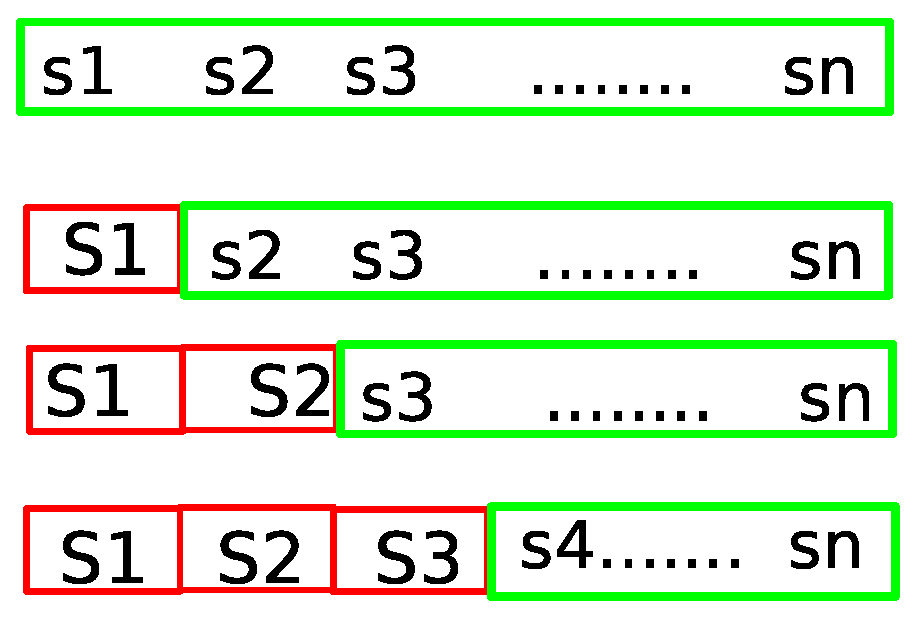
\includegraphics[width=3in] {L7-incremental-dc.eps}
%\end{figure}
%}


\frame[allowframebreaks]{
\frametitle{If a problem can be reduced into smaller sub-problems}

\begin{itemize}
\item 
There are two possible solving strategies: 
\begin{enumerate}
 \item \textcolor{red}{\bf Incremental}: to solve the original problem, it suffices to solve a smaller sub-problem; thus the problem  is shrunk step-by-step. In other words, a feasible solution can be  constructed step-by-step. \\
  For example, in  Gale-Shapley
algorithm,  the final complete solution is constructed step by step, and a {\bf stable, partial} matching is 
maintained during the construction process.  

\begin{figure} 
  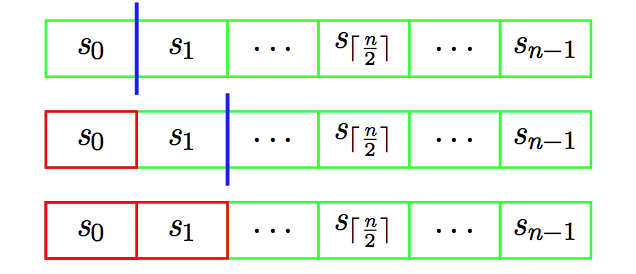
\includegraphics[width=3in]{L5-incremental-dc1.png}
\end{figure}


 \item \textcolor{red}{\bf divide-and-conquer}: the original problem is decomposed into several independent sub-problems; thus, a feasible solution to the original problem can be constructed by assembling the solutions to independent sub-problems. 
\begin{figure} 
  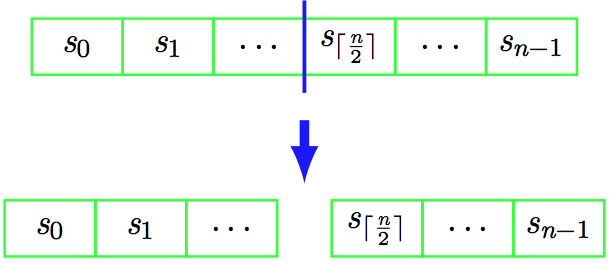
\includegraphics[width=3in]{L5-incremental-dc2.png}
\end{figure}

\end{enumerate}
\end{itemize} 

}


\frame{
\begin{block}{}
 The first example: Two versions of {\sc IntervalScheduling} problem
\end{block}
}


\frame{
\frametitle{ {\sc IntervalScheduling} problem }
\begin{itemize} 
\item 
Practical problem: 
	\begin{itemize}
	\item a class room is requested by several courses; 
	\item the $i$-th course $A_i$ starts from  $S_i$ and ends at $F_i$.
	\end{itemize}
\item  Objective: to meet as many students as possible. 
 \end{itemize}
 } 
 
\frame{
\frametitle{ An instance } 
Example: \\
\begin{figure}
 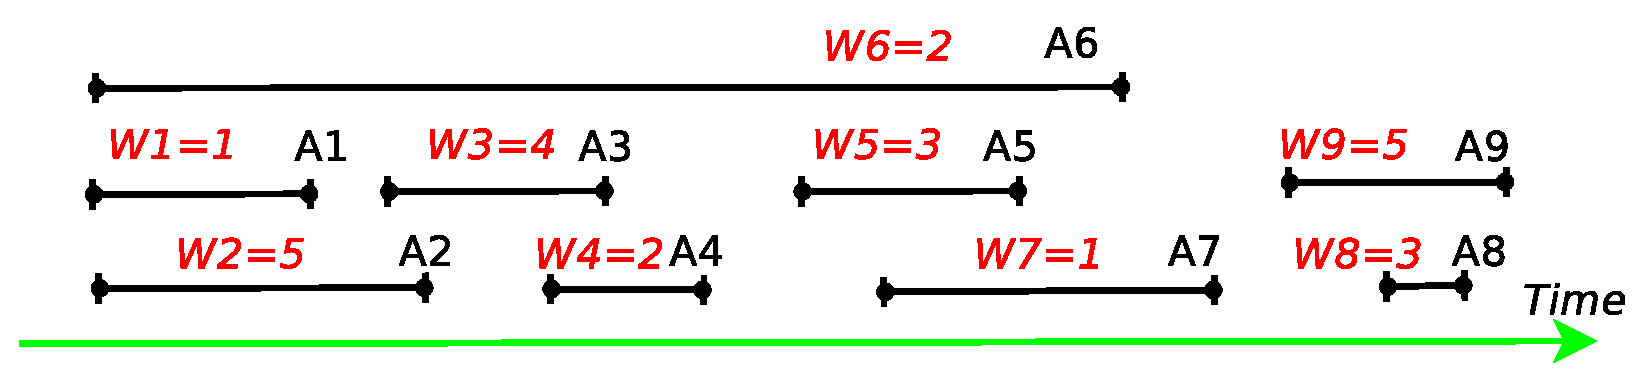
\includegraphics[width=4in] {L7-intervalschedulingexample.eps}
\end{figure}

\begin{eqnarray}  \nonumber
\texttt{Solutions:} & S_1=\{ A_1, A_3, A_5, A_8 \} &|\quad S_2= \{ A_6, A_9 \}  \nonumber \\
\texttt{Benefits:} &  B(S_1)=1+4+3+3=11 &|\quad  B(S_2)=2+5=7   \nonumber 
\end{eqnarray} \nonumber
}

 
\frame{
\frametitle{ {\sc IntervalScheduling} problem: version 1 }
 
 	\begin{itemize}
	\item 
 Formulation: 
\begin{block}{}
{\bf INPUT: }  \\
  $n$ activities $A=\{A_1, A_2, ..., A_n \}$ that wish to use a resource. Each activity $A_i$ uses the resource during interval $[S_i, F_i)$. The selection of activity $A_i$ yields a benefit of $W_i$.\\
{\bf OUTPUT: } \\ 
 To select a collection of \textcolor{blue}{\bf compatible} activities to \textcolor{red}{\bf maximize benefits}.  
\end{block}

		\item Here, $A_i$ and $A_j$ are \textcolor{blue}{\bf compatible} if there is no overlap between the corresponding intervals $[S_i, F_i)$ and $[S_j, F_j)$, i.e. the resource cannot be used by more than one activities at a time.
		\item It is assumed that the activities have been sorted according to the finishing time, i.e. $F_i \leq F_j$ for any $i < j$. 
	\end{itemize}
}


\frame[allowframebreaks]{
\frametitle{Key observation}
\begin{itemize}
\item It is not easy to solve a problem with $n$ activities directly. Let's see whether it can be reduced into smaller sub-problems. 
\item Solution: a subset of activities. Imagine the solving process as a series of decisions; at each  decision step, we choose an activity to use the resource.  
\item Suppose we have already worked out the optimal solution. Consider \textcolor{red}{\bf the first  decision} in the optimal solution, i.e. whether $A_n$ is selected or not. There are $2$ options: 
\ \\
\begin{enumerate}
 \item Select activity $A_n$: the selection leads to a  \textcolor{red}{\bf smaller subproblem}, namely selecting from the activities ending before $S_n$. 
 \begin{figure}
 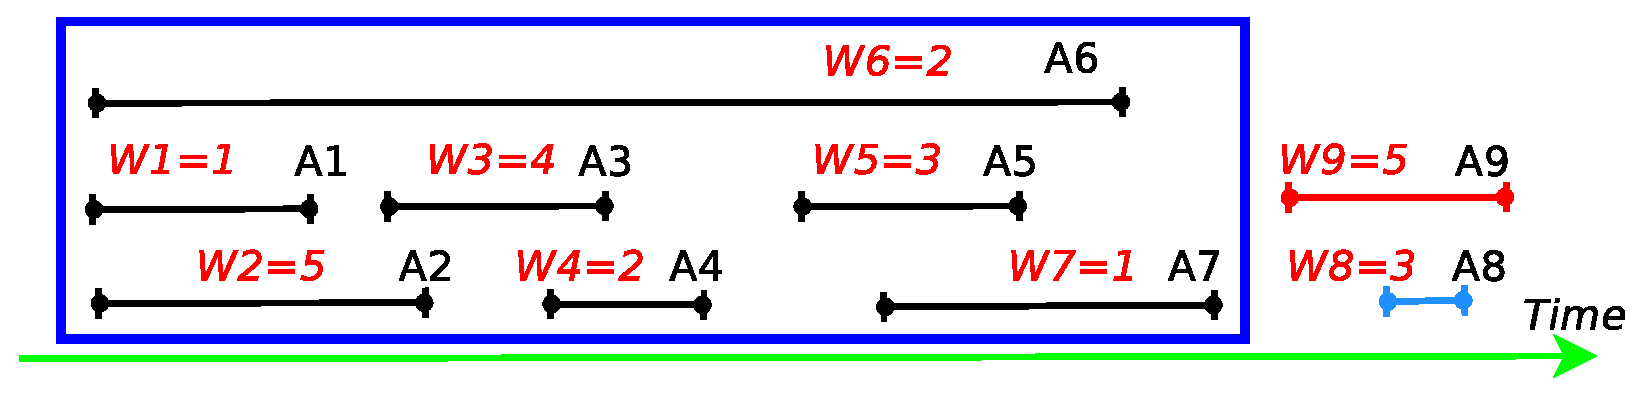
\includegraphics[width=3in] {L7-intervalschedulingexamplek1.eps}
\end{figure}
 \item Abandon activity $A_n$: then it suffices to solve another \textcolor{red}{\bf smaller subproblem}: to select activities from $A_1, A_2, ..., A_{n-1}$. 
  \begin{figure}
 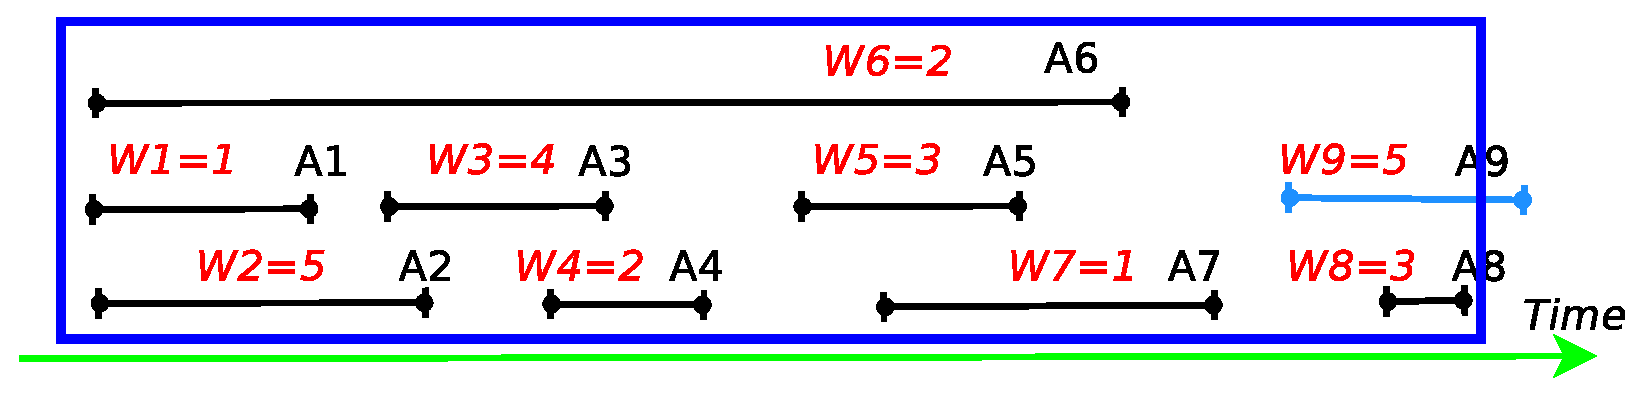
\includegraphics[width=3in] {L7-intervalschedulingexamplek2.eps}
\end{figure}
 \end{enumerate}

\end{itemize}
} 


\frame{
\frametitle{Key observation cont'd}
% \begin{figure}
% 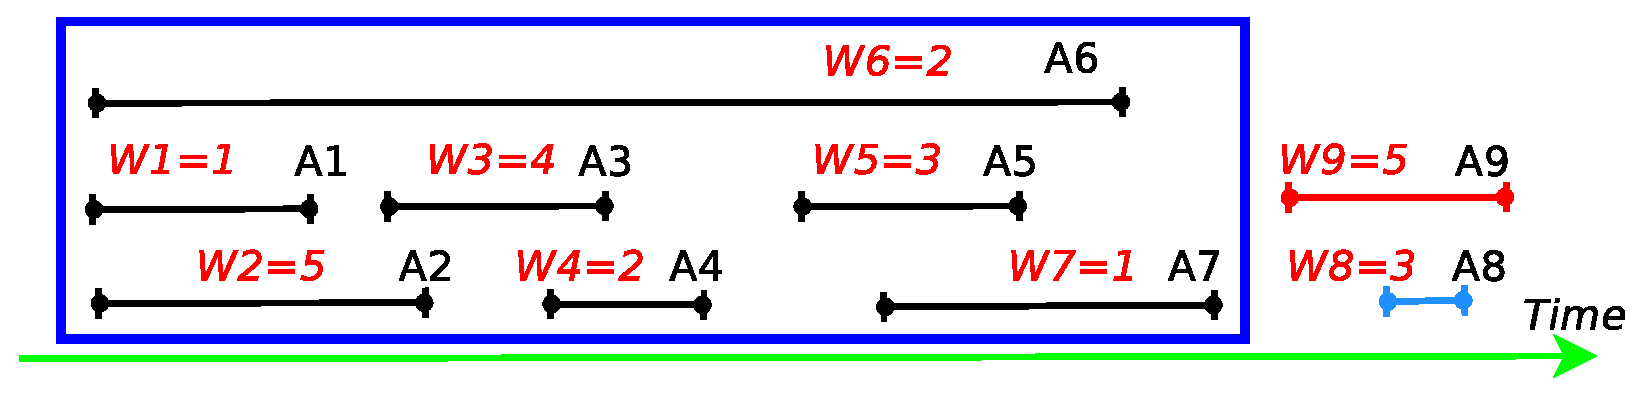
\includegraphics[width=4in] {L7-intervalschedulingexamplek1.eps}
%\end{figure}
%
%  \begin{figure}
% 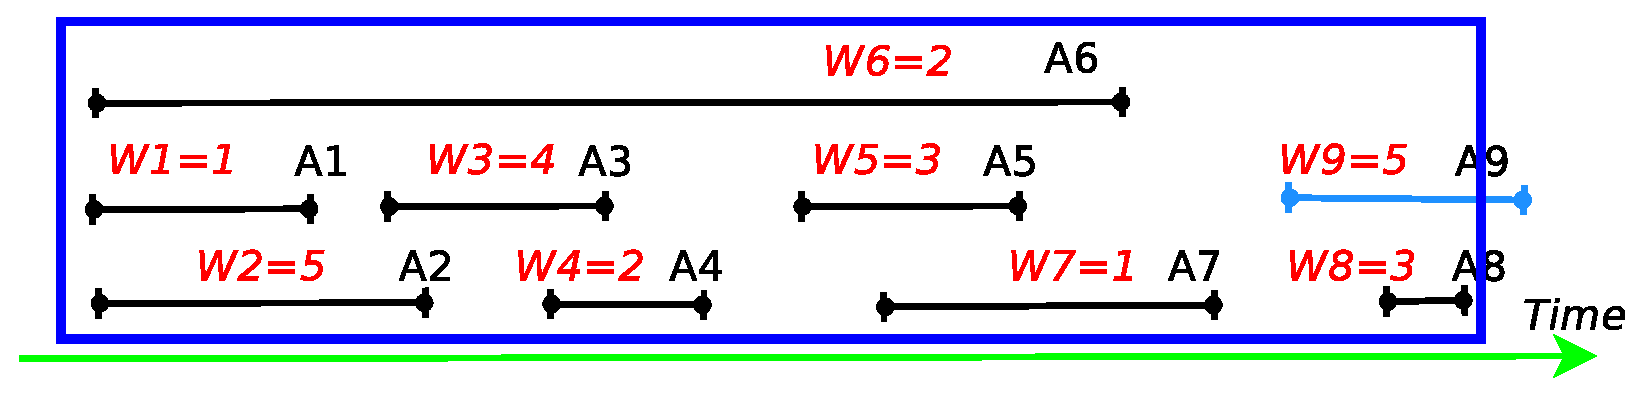
\includegraphics[width=4in] {L7-intervalschedulingexamplek2.eps}
%\end{figure}


\begin{itemize}
\item Summarizing the two cases,  we can design the general form of subproblems as: \\
\textcolor{red}{ {\bf selecting a collection of activities from $A_1, A_2, ..., A_i$ to maximize benefits}}. 
%\footnote{  $A_{i..j} = \phi$ whenever $i\geq j$. Here we suppose that  all $A_i$ were sorted in increasing order of finish time, and $A_0$ and $A_{10}$ are introduced as a sentinels. }
%\item Intuition of $A_{i..j}$: the activities begin after $A_i$ ends and end before $A_j$ starts. 

%\item Intuition of $A_{i..j}$: the activities begin after $A_i$ ends and end before $A_j$ starts. 
\item  Denote the optimal solution value as $OPT(i)$. 
\item Optimal substructure property: (``cut-and-paste'' argument)
  $OPT(i) = \max \begin{cases}
        OPT( pre(i) ) + W_i \nonumber \\ 
  	OPT( i-1) \nonumber 
  \end{cases} 
  $   \\
Here, $pre(i)$ denotes the largest index of the activities ending before $S_i$. 
\end{itemize}
}



\frame{
\frametitle{ Dynamic programming algorithm} 
\begin{footnotesize}
{\sc Recursive\_DP}$( i )$
\begin{algorithmic}[1]
\REQUIRE{ All $A_i$ have been sorted in the increasing order of $F_i$.}
\IF { $i \leq 0$ } 
	\RETURN $0$; 
\ENDIF
\IF { $i == 1$ } 
	\RETURN $W_1$; 
\ENDIF
\STATE Determine the largest index of the activities ending before $S_i$, denoted as  $pre(i)$. 
\STATE $m=  \max \begin{cases}
        \text{\sc Recursive\_DP}( pre(i) ) + W_i \nonumber \\ 
  	\text{\sc Recursive\_DP}( i-1) \nonumber 
  \end{cases} $  
\RETURN $m$;
\end{algorithmic}
\end{footnotesize}
Note: \\
\begin{itemize}
\item The original problem can be solved by calling {\sc Recursive\_DP}$(n)$. 
\item It needs $O(n \log n)$ to sort the activities and determine $pre(.)$, and the dynamic programming needs $O(n)$ time. 
\item   Thus, time complexity: $O(n \log n)$
\end{itemize}
}


\frame{
	\begin{block}{}
	{\sc IntervalScheduling} problem: version 2
	\end{block}
}

\frame{
\frametitle{ Let's investigate a special case }

\begin{figure}
 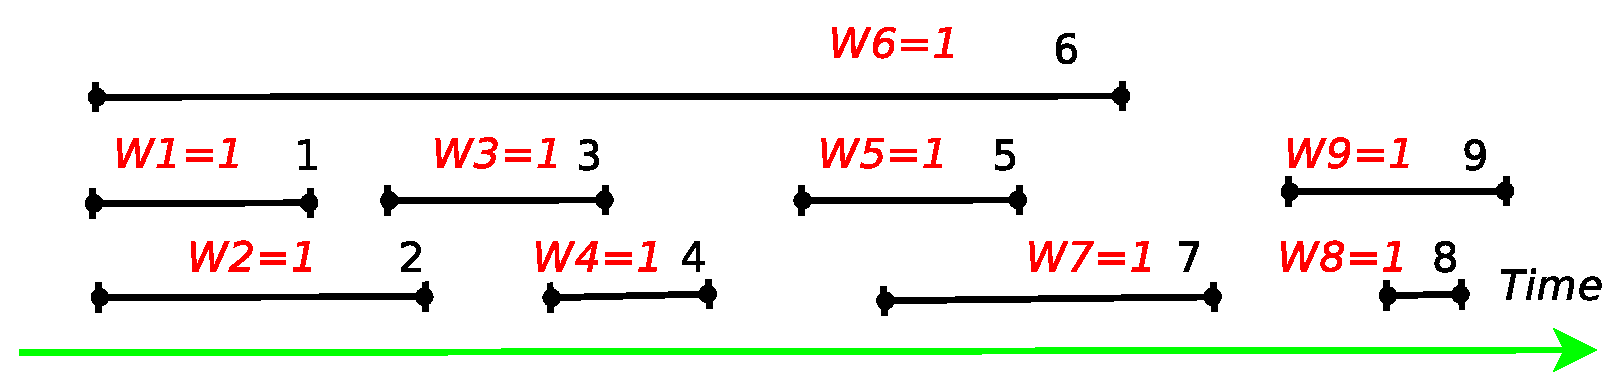
\includegraphics[width=4in] {L7-intervalschedulingexampleall1.eps}
\end{figure}
A special case of {\sc IntervalScheduling} problem with \textcolor{red}{\bf all weights $w_i=1$}. \\

} 

\frame{
\frametitle{ {\sc IntervalScheduling} problem: version 2  }
 Formulation: 
\begin{block}{}
{\bf INPUT: }  \\
  $n$ activities $A=\{A_1, A_2, ..., A_n \}$ that wish to use a resource. Each activity $A_i$ uses the resource during interval $[S_i, F_i)$. \\
{\bf OUTPUT: } \\ 
To select as many \textcolor{blue}{\bf compatible activities} as possible.
\end{block}

}

\frame{
 
\begin{block}{}
Greedy selection property
\end{block}

}



\frame[allowframebreaks]{
\frametitle{Another key observation: Greedy selection }
\begin{itemize}
\item Since this is just a special case, the \textcolor{red}{\bf optimal substructure property}  still holds.
\item Besides the optimal substructure property, the special weight setting leads to \textcolor{red}{\bf ``greedy selection'' property}.
\end{itemize}


\begin{Theorem}
Suppose $A_1$ is the activity with the earliest ending time.  \textcolor{red}{\bf $A_1$ is used in an optimal solution. }
\end{Theorem}
\begin{Proof} (exchange argument) \\
\begin{itemize}
 \item 
Suppose we have an optimal solution $O = \{ A_{i1}, A_{i2}, ..., A_{iT} \}$ but $A_{i1} \neq A_m$. \\
\item $A_1$ ends earlier than $A_{i1}$. \\
\item $A_1$ is compatible with $A_{i2}, ..., A_{iT}$. (Why?) \\
\item Construct a new subset $O' = O - \{A_{i1} \} \cup \{ A_1 \} $ \\
\item $O'$ is also an optimal solution since $| O' | = | O | $. 
\end{itemize}
\begin{figure}
 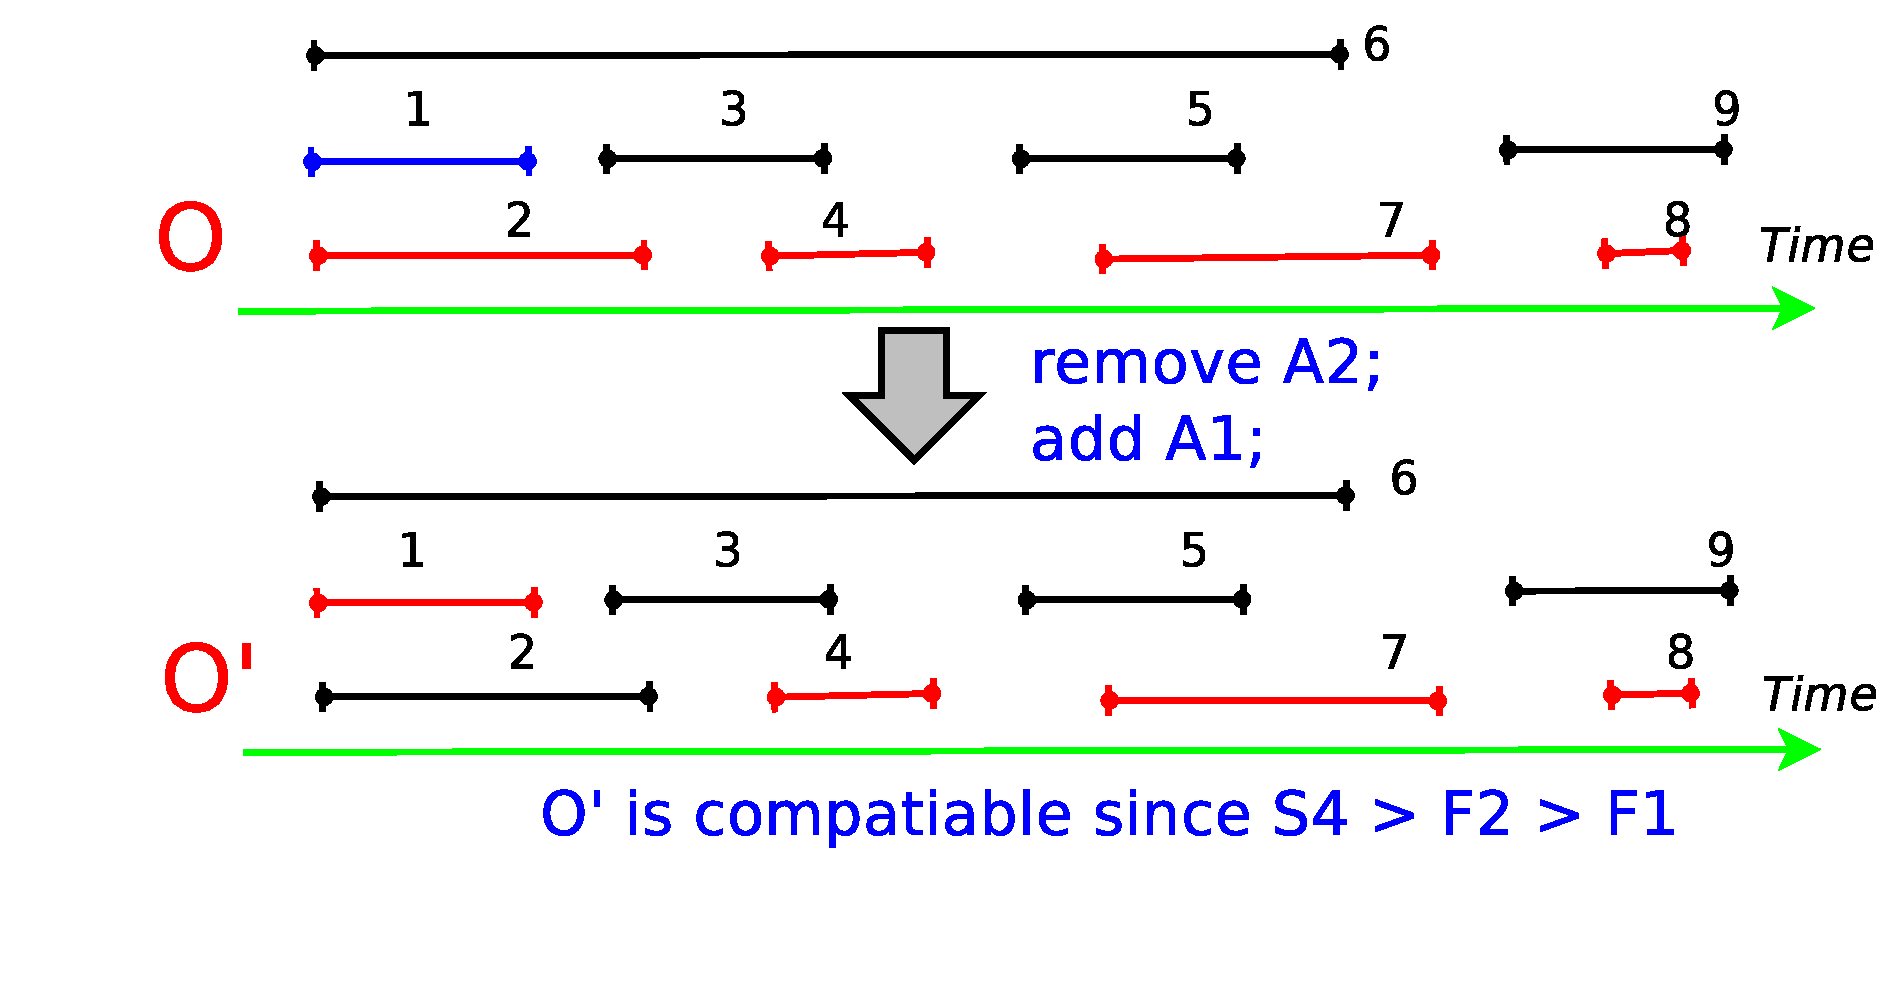
\includegraphics[width=2.9in] {L7-intervalschedulingexampleall1am.eps}
\end{figure}
\end{Proof}
}

\frame{
\frametitle{Simplifying the DP algorithm into a greedy algorithm }

{\sc Interval\_Scheduling\_Greedy}$( n )$
\begin{algorithmic}[1]
\REQUIRE{ All $A_i$ have been sorted in the increasing order of $F_i$.}
\STATE $previous\_finish\_time=-\infty;$
\FOR{ $i=1$ to $n$ }
\IF { $S_i \geq  previous\_finish\_time$ }
\STATE{ Select activity $A_i$;}
\STATE $previous\_finish\_time = F_i;$
\ENDIF
\ENDFOR
\end{algorithmic}

Time complexity: $O(n\log n)$ (sorting activities in the increasing order of finish time).
%\item We can improve the algorithm  in a top-down fashion, rather than the bottom-up manner typically used in DP. 

} 



% \frame[allowframebreaks]{
% \frametitle{Simplifying the dynamic programming algorithm to greedy algorithm }
% 
%  \begin{figure}%
%      \begin{minipage}{0.32\textwidth}%
%       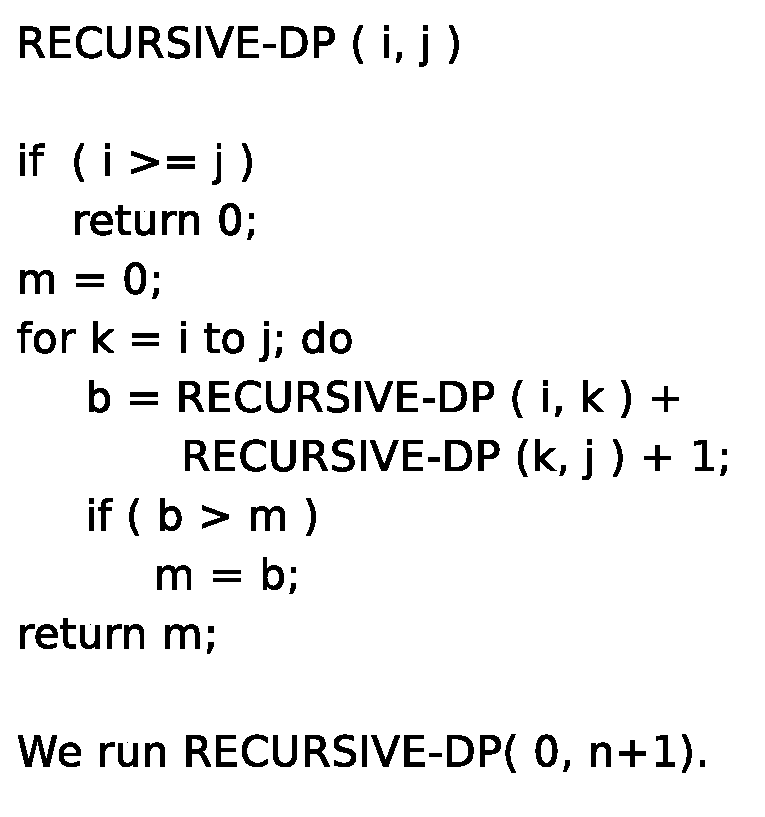
\includegraphics[width=1.0\textwidth]{L7-intervalschedulingdpalgo.eps}%
%      \end{minipage}%
%  \quad
%      \begin{minipage}{0.30\textwidth}
%       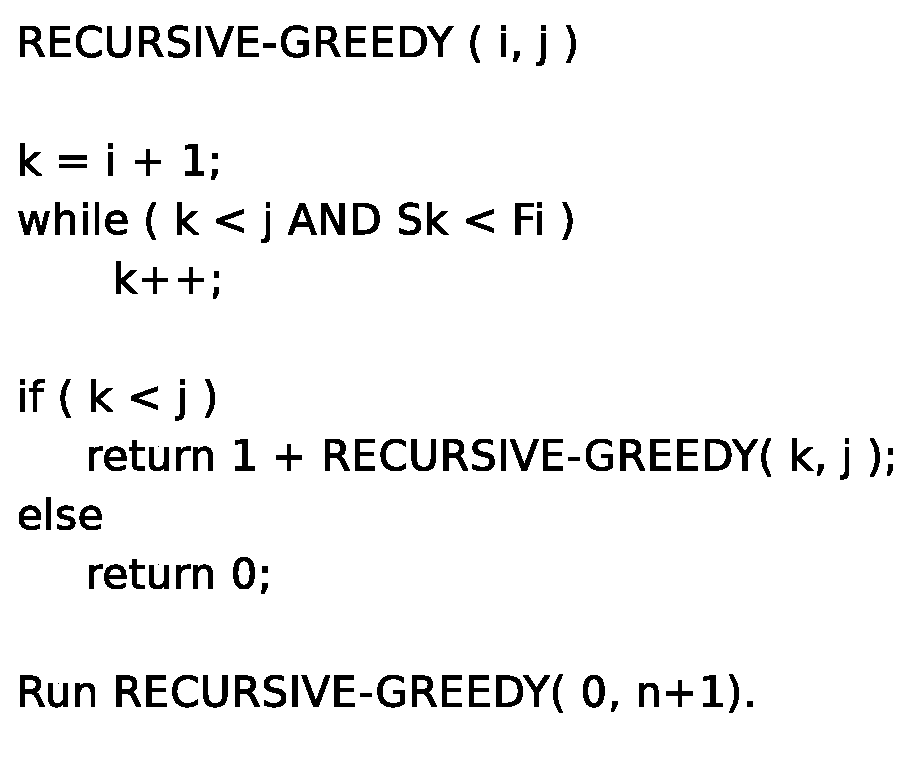
\includegraphics[width=1.0\textwidth]{L7-intervalschedulinggreedyalgo.eps}%
%      \end{minipage}%
%  \quad
%       \begin{minipage}{0.25\textwidth}
%       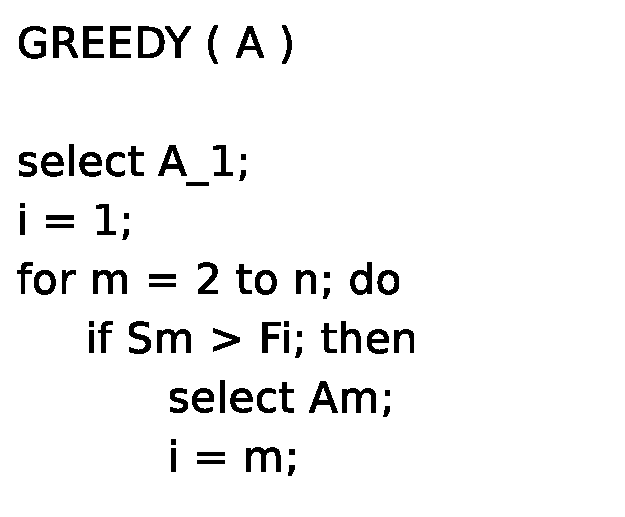
\includegraphics[width=1.0\textwidth]{L7-intervalschedulinggreedyalgo2.eps}%
%      \end{minipage}%
% 
%  \end{figure}
% 
% DP algorithm:  we have $j-i-1$ options when solving $A_{i..j}$, and a choice yields two subproblems.  \\
% Time-complexity: $O(n^3)$.       
% }
% 
% \frame[allowframebreaks]{
% \frametitle{Simplifying the dynamic programming algorithm to greedy algorithm }
% 
%  \begin{figure}%
%      \begin{minipage}{0.32\textwidth}%
%       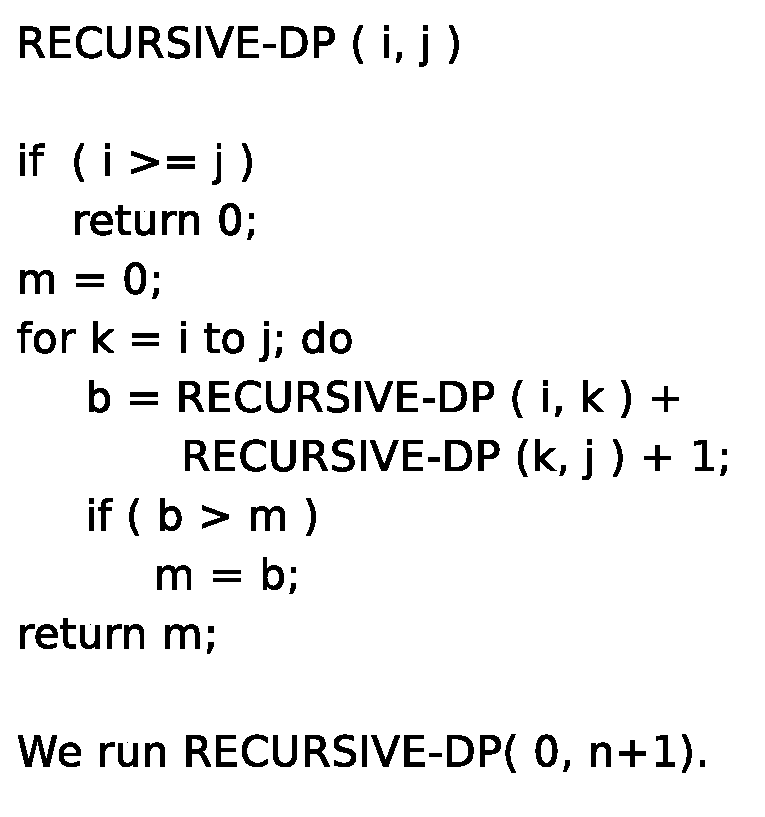
\includegraphics[width=1.0\textwidth]{L7-intervalschedulingdpalgo.eps}%
%      \end{minipage}%
%  \quad
%      \begin{minipage}{0.30\textwidth}
%       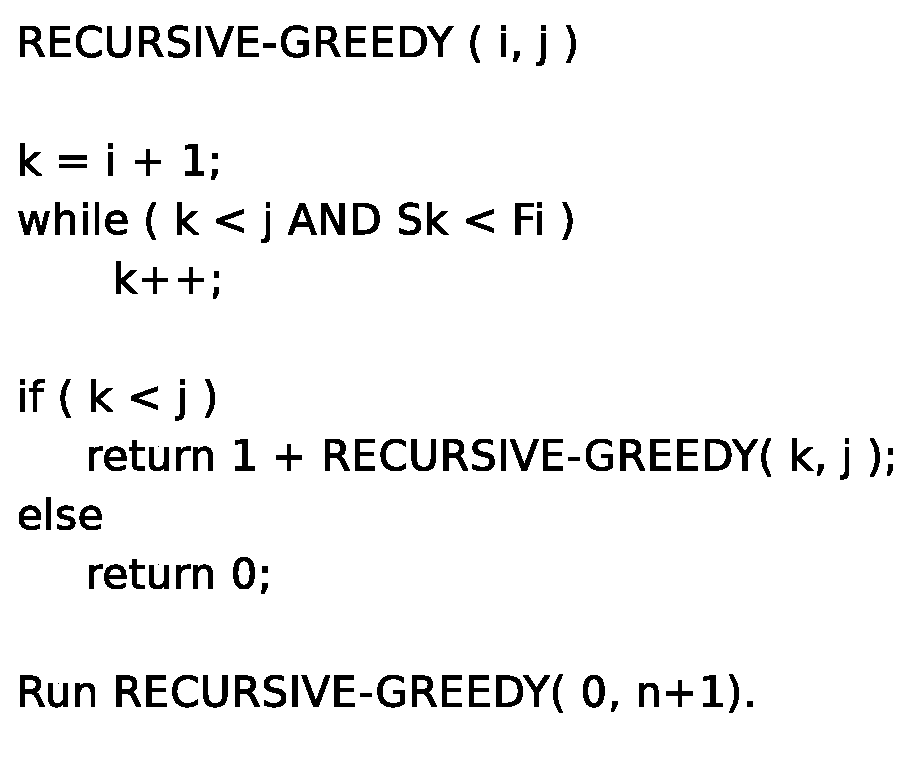
\includegraphics[width=1.0\textwidth]{L7-intervalschedulinggreedyalgo.eps}%
%      \end{minipage}%
%  \quad
%       \begin{minipage}{0.25\textwidth}
%       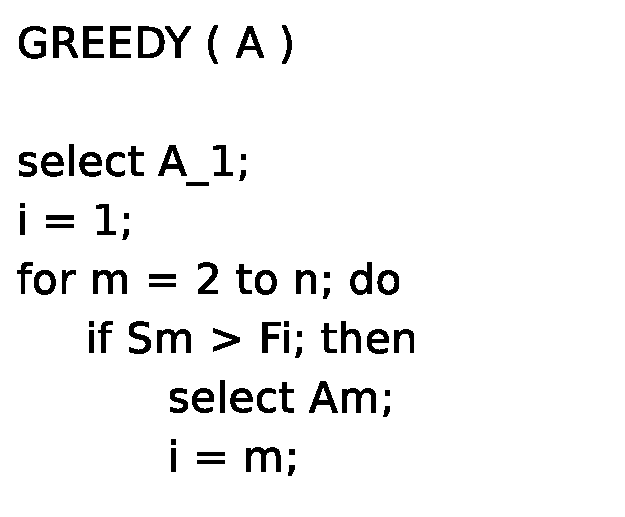
\includegraphics[width=1.0\textwidth]{L7-intervalschedulinggreedyalgo2.eps}%
%      \end{minipage}%
% 
%  \end{figure}
% 
% Greedy algorithm:  only one option (greedy selection), and the subproblem $A_{ik}$ is empty. Thus choosing $A_k$ leads to only one subproblem. \\
% Time-complexity: $O(n \log n )$. 
% }
% 
% \frame[allowframebreaks]{
% \frametitle{Simplifying the dynamic programming algorithm to greedy algorithm }
% 
%  \begin{figure}%
%      \begin{minipage}{0.32\textwidth}%
%       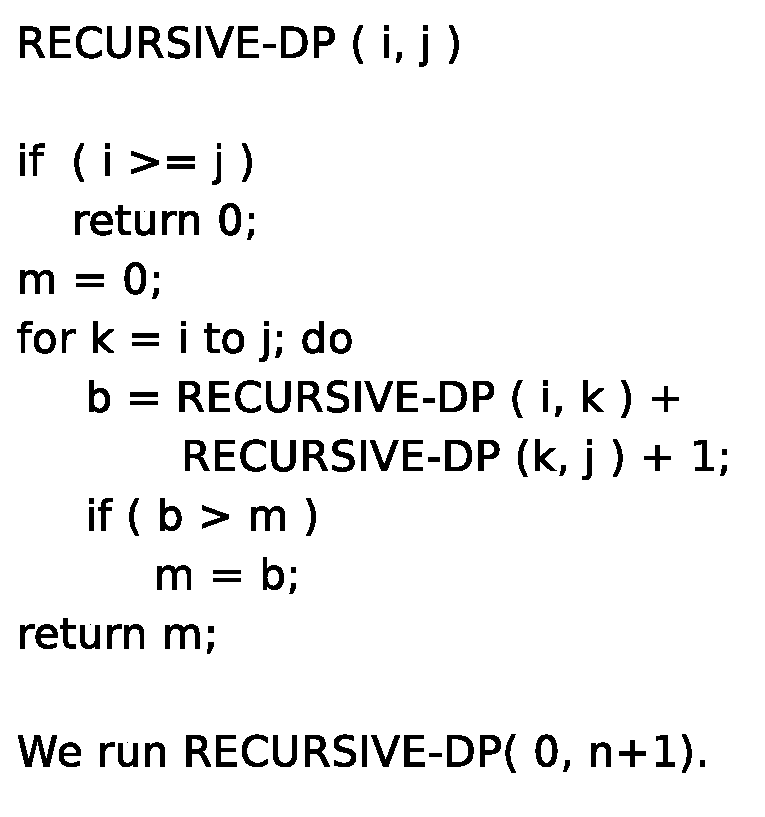
\includegraphics[width=1.0\textwidth]{L7-intervalschedulingdpalgo.eps}%
%      \end{minipage}%
%  \quad
%      \begin{minipage}{0.30\textwidth}
%       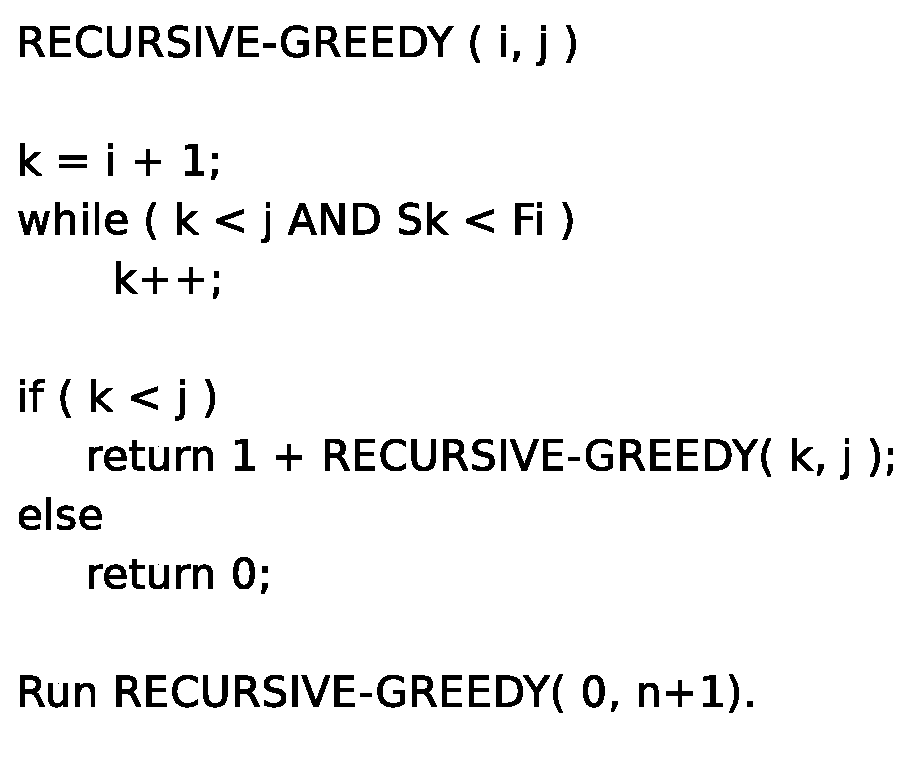
\includegraphics[width=1.0\textwidth]{L7-intervalschedulinggreedyalgo.eps}%
%      \end{minipage}%
%  \quad
%       \begin{minipage}{0.25\textwidth}
%       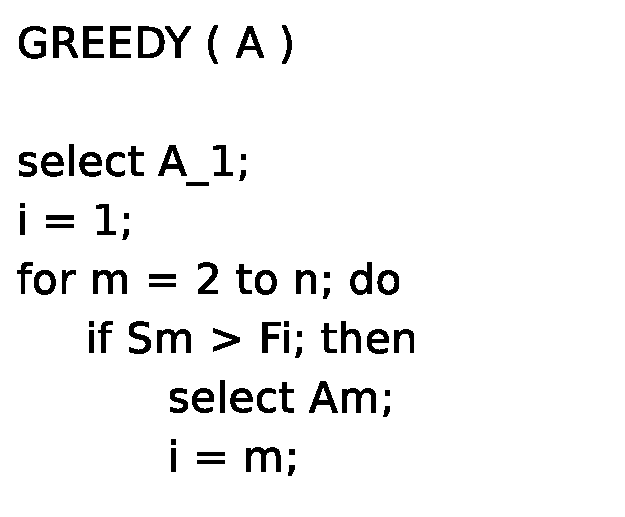
\includegraphics[width=1.0\textwidth]{L7-intervalschedulinggreedyalgo2.eps}%
%      \end{minipage}%
% \end{figure}
% We can solve each subproblem in a top-down fashion, rather than a bottom-up manner typically used in DP.  
% }

\frame[allowframebreaks]{
\frametitle{An example } 
Step 1: 
\begin{figure}
 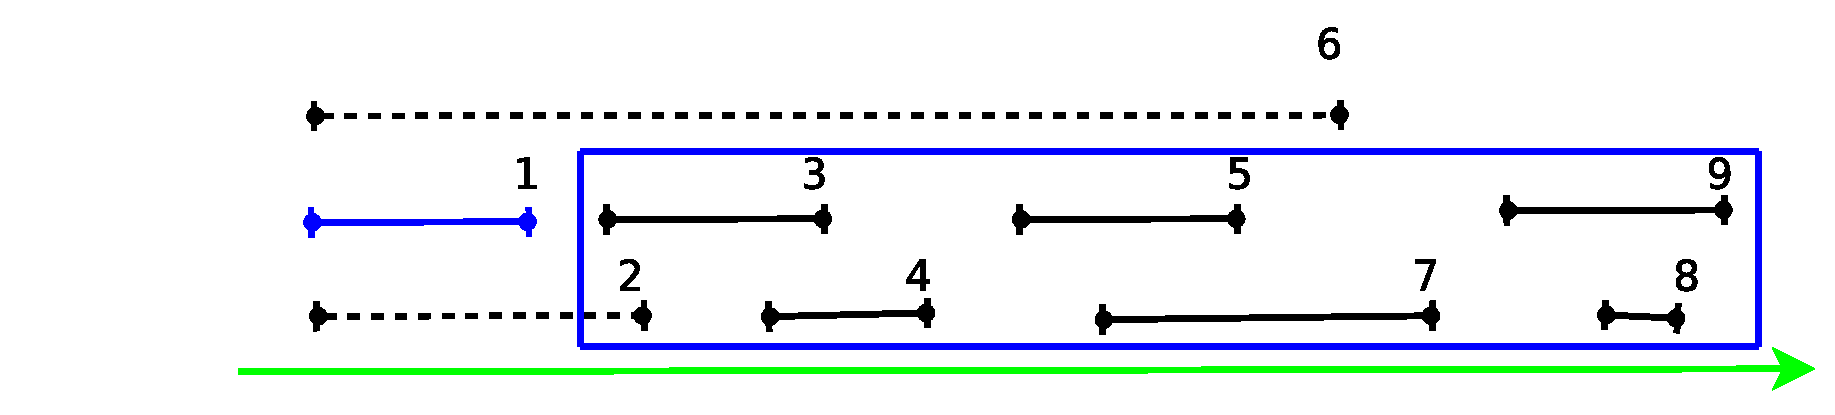
\includegraphics[width=4.1in] {L7-intervalschedulingexamplegreedystep1.eps}
\end{figure}

Step 2: 
\begin{figure}
 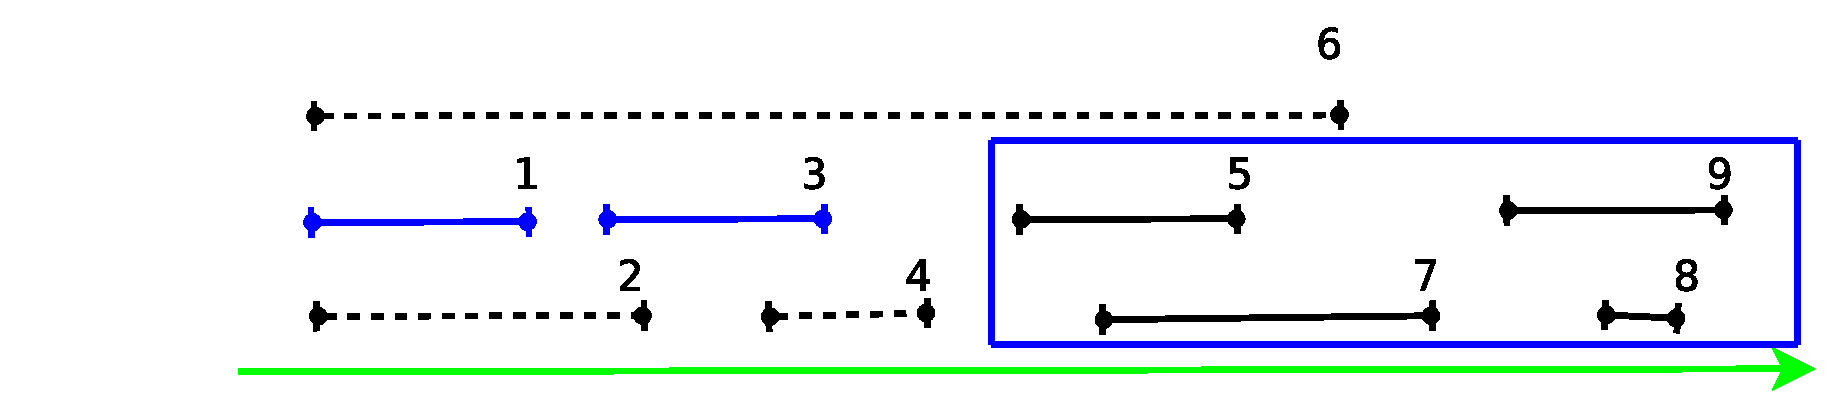
\includegraphics[width=4.1in] {L7-intervalschedulingexamplegreedystep2.eps}
\end{figure}

\ \\
\ \\
Step 3: 
\begin{figure}
 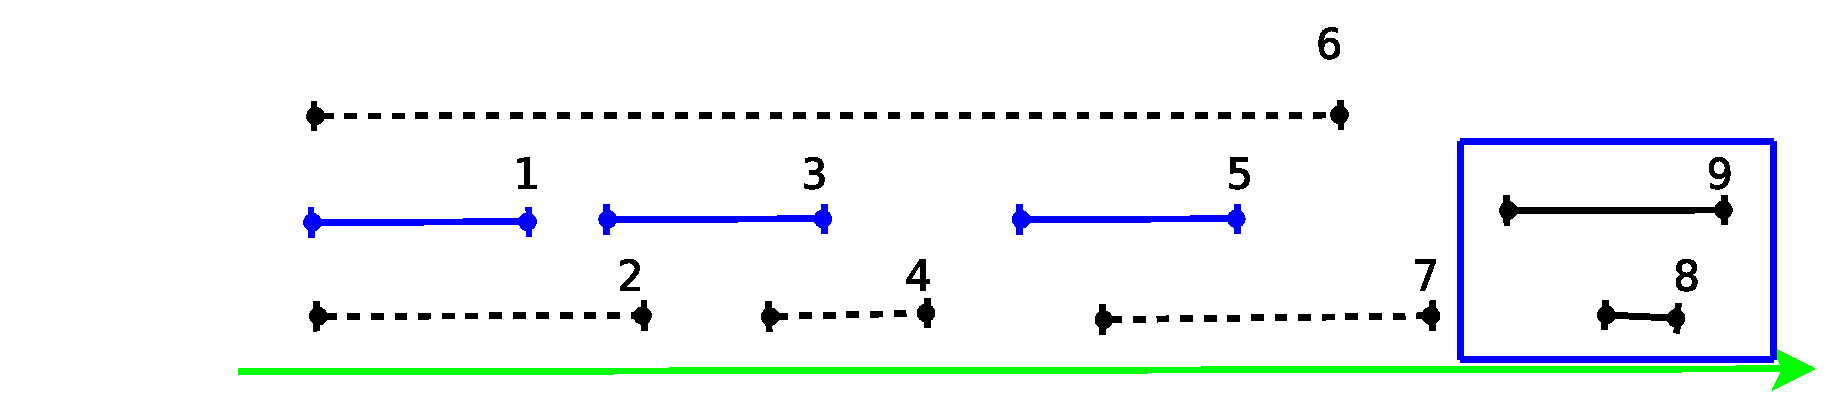
\includegraphics[width=4in] {L7-intervalschedulingexamplegreedystep3.eps}
\end{figure}

Step 4: 
\begin{figure}
 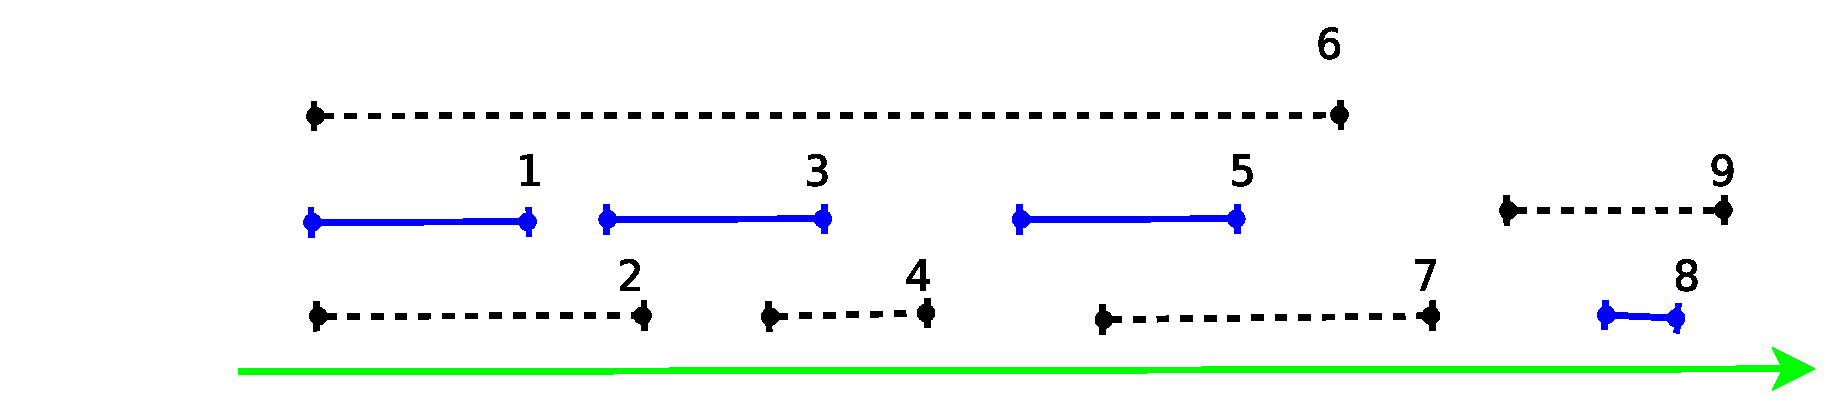
\includegraphics[width=4in] {L7-intervalschedulingexamplegreedystep4.eps}
\end{figure}

(see another demo) 
}

%\frame{
%\frametitle{Analysis  }
%
%\begin{itemize}
%\item 
%
% \item 
%  Unlike \textcolor{blue}{\bf enumerating all possible options} in DP, it suffices to use \textcolor{blue}{\bf only one option},  i.e. greedy selection,  at each decision step. Thus, the sub-problem $A_{ik}$ is {\it null}  and only one sub-problem is left. 
%\item Notice that the greedy selection is determined without knowledge of solutions to subproblems. 
%\end{itemize}
%}

\frame{
	\begin{block}{}
		Question: does the greedy algorithm work in  general cases?
	\end{block}
}

\frame{
\frametitle{ Why greedy strategy doesn't work for the general {\sc IntervalScheduling} problem? }
\begin{figure}
 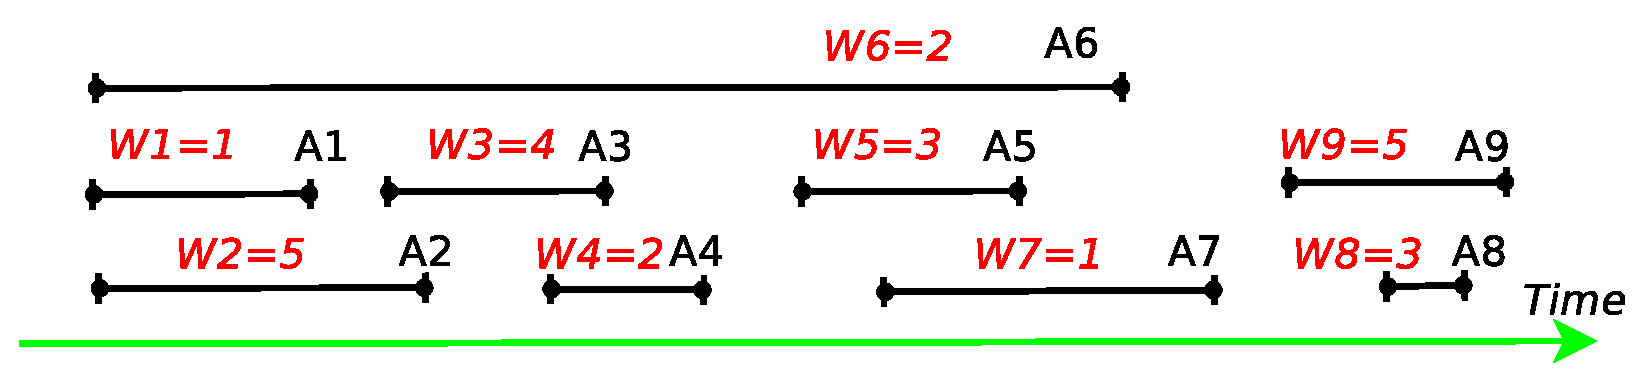
\includegraphics[width=4in] {L7-intervalschedulingexample.eps}
\end{figure}
\begin{footnotesize}
\begin{eqnarray}
\texttt{Solutions:} & Greedy: \{ A_1, A_3, A_5, A_8 \} &|\quad  OPT: \ \{ A_2, A_4, A_5, A_9 \}  \nonumber \\
\texttt{Benefits:} &  1+4+3+3=11 & |\quad   5+2+3+5=15   \nonumber 
\end{eqnarray}
\end{footnotesize}
\begin{itemize}
\item 
Reason: Greedy choice property doesn't hold. 
\item 
Note: although the problem is the same, a slight change of weights leads to significant affects on algorithm design.
\end{itemize}
}


\frame{
\frametitle{ DP versus Greedy }
Similarities: 
\begin{enumerate}
\item
Both dynamic programming and greedy techniques are typically applied to \textcolor{red}{\bf optimization} problems. 
\item \textcolor{red}{\bf Optimal substructure}: Both dynamic programming and greedy techniques exploit the optimal substructure property. 
\item \textcolor{blue}{ {\bf Beneath every greedy algorithm, there is almost always a more cumbersome dynamic programming solution \quad --- CRLS} }
\end{enumerate}

} 

\frame{
\frametitle{ DP versus Greedy  cont'd}

Differences: 
\begin{enumerate}
 \item A dynamic programming method typically \textcolor{red}{\bf enumerate all possible options at a decision step}, and the decision cannot be determined before subproblems were solved.
 \item In contrast, greedy algorithm does not need to enumerate all possible options---it simply \textcolor{red}{\bf make a locally optimal (greedy) decision} without considering results of subproblems. 
\end{enumerate}
Note: 
\begin{itemize}
	\item Here, ``\textcolor{red}{local}'' means that we have already acquired part of an optimal solution, and the partial knowledge of optimal solution is sufficient to help us make a wise decision. 
	\item Sometimes a rigorous proof is unavailable, thus extensive experimental results are needed to show the efficiency of the greedy technique. 
\end{itemize}

}

%\frame{
%\frametitle{ How to design greedy method?} 
%Two strategies:
%\begin{enumerate}
% \item Simplifying a dynamic programming method through greedy selection;
% \item Trial-and-error: Imagining the solution-generating process as making a sequence of choices, and trying different greedy selection rules.
%\end{enumerate}
%
%
%}

\frame{
	\begin{block}{}
		Trying other greedy rules 
	\end{block} 
}

\frame{
\frametitle{ Incorrect trial 1: {\bf earlist start} rule } 
\begin{itemize}
\item Intuition: the earlier start time, the better.   
\item Incorrect. A negative example: 
\begin{figure}
 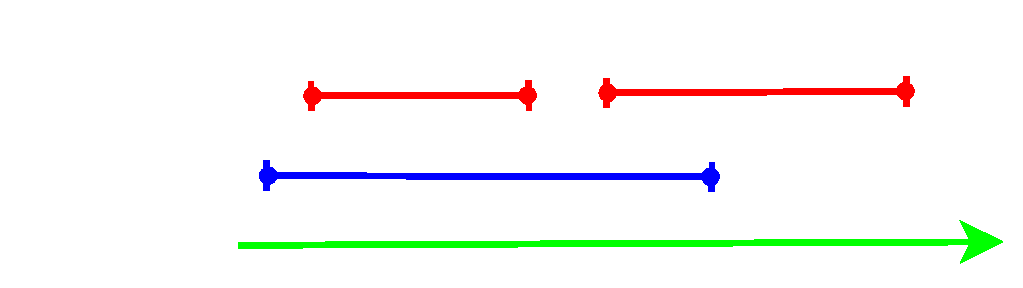
\includegraphics[width=2in] {L7-intervalschedulingexample-error2.eps}
\end{figure}

 \item 
Greedy solution: blue one. Solution value: 1. 
\item 
Optimal solution: red ones. Solution value: 2.
\end{itemize}
}

\frame{
\frametitle{ Incorrect trial 2: trying {\bf minimal duration } rule } 
\begin{itemize}
\item Intuition: the shorter duration, the better. 
\item Incorrect. A negative example: 
\begin{figure}
 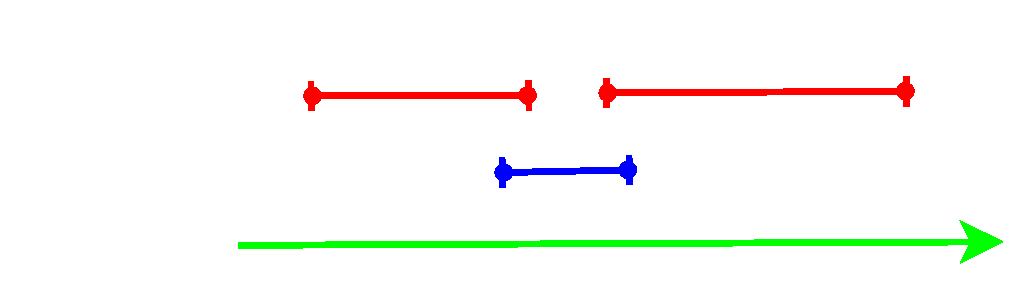
\includegraphics[width=2in] {L7-intervalschedulingexample-error1.eps}
\end{figure}

 \item 
Greedy solution: blue one. Solution value: 1. 
\item 
Optimal solution: red ones. Solution value: 2.
\end{itemize}
}


\frame{
\frametitle{ Incorrect trial 3: trying {\bf minimal conflicts } rule } 
\begin{itemize}
\item Intuition: the less conflict activities, the better. 
\item Incorrect. A negative example: 
\begin{figure}
 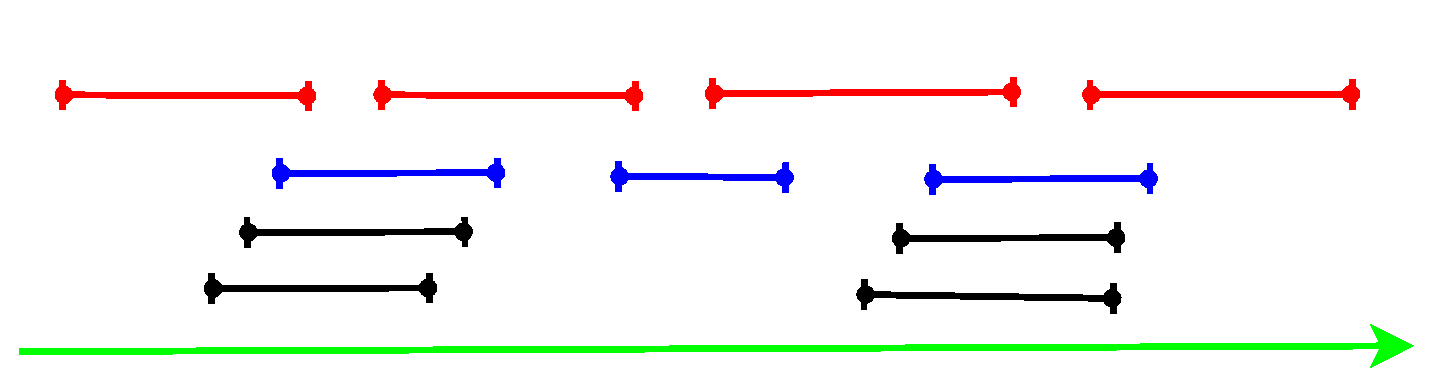
\includegraphics[width=3in] {L7-intervalschedulingexample-error3.eps}
\end{figure}
 \item 
Greedy solution: blue ones. Solution value: 3. 
\item 
Optimal solution: red ones. Solution value: 4.
\end{itemize}
}

\frame{
	\frametitle{Elements of greed strategy}
	\begin{itemize}
		\item A greedy algorithm makes ``locally optimal" choice at each stage with 
		a hope of finding ``global optimum". 
		\item Key components of a greedy algorithm: 
			\begin{enumerate}
				\item A candidate set: from which a solution is created;
				\item A selection rule: to choose the best candidate to add to a partial solution;
				\item An objective function: to assign a value to both complete solution, and partial solution; 
				\item A solution function: to indicate whether we have already obtained a complete solution. 
			\end{enumerate}

	\end{itemize}
}

\frame{
	\frametitle{Partial solution tree}
	\begin{itemize}
		\item Suppose the feasible solutions have the form $X = [x_1, x_2, ..., x_n ]$, and $x_i \in S_i$, and the objective is to find $X^*$ such that $f(X^*)$ is an optimum. 
		\item Let's construct the \textcolor{red}{\bf partial solution tree} first.

 \begin{figure}
\begin{tikzpicture}[scale=1., auto,swap]
    % Draw a 7,11 network
    % First we draw the vertices
    \foreach \pos/\name in {{(0,0)/A1234}, {(-1,-1)/A12}, {(1,-1)/A34}, {(-1.5,-2)/A1}, {(-.5, -2)/A2}, {(0.5, -2)/A3}, {(1.5, -2)/A4}}
        \node[smallvertex,draw=black, fill=blue!20] (\name) at \pos {};
    % Connect vertices with edges and draw weights
    \foreach \source/ \dest /\weight in {A1234/A12/{}, A1234/A34/{}, A12/A1/{}, A12/A2/{}, A34/A3/{}, A34/A4/{}  }
        \path[undirectededge] (\source) -- node[weight] {$\weight$} (\dest);
%       \draw[dashed, ->] (0,0) arc  (120:60:2);
 
   \node[above] at (0,0.2) {\tiny $ \Phi $};
   \node[left] at (-1.2, -1) {\tiny $ [0] $};
   \node[right] at (1.2, -1) {\tiny $ [1]$};
   \node[below] at (-1.5, -2.2) {\tiny $ [0, 0]$};
   \node[below] at (-.5, -2.2) {\tiny $[0, 1]$};
   \node[below] at (.5, -2.2) {\tiny $[1, 0]$};
   \node[below] at (1.5, -2.2) {\tiny $[1, 1]$};
   \end{tikzpicture}
\end{figure}
	\item Each internal node denotes a ``partial solution", and a leaf denote a ``complete solution". Note that each node is associated with a value. 
	\end{itemize}
} 

\frame{
	\frametitle{ Enumeration vs. greedy}
 \begin{figure}
\begin{tikzpicture}[scale=1., auto,swap]
    % Draw a 7,11 network
    % First we draw the vertices
    \foreach \pos/\name in {{(0,0)/A1234}, {(-1,-1)/A12}, {(1,-1)/A34}, {(-1.5,-2)/A1}, {(-.5, -2)/A2}, {(0.5, -2)/A3}, {(1.5, -2)/A4}}
        \node[smallvertex,draw=black, fill=blue!20] (\name) at \pos {};
    % Connect vertices with edges and draw weights
    \foreach \source/ \dest /\weight in {A1234/A12/{}, A1234/A34/{}, A12/A1/{}, A12/A2/{}, A34/A3/{}, A34/A4/{}  }
        \path[undirectededge] (\source) -- node[weight] {$\weight$} (\dest);
%       \draw[dashed, ->] (0,0) arc  (120:60:2);
 
   \node[above] at (0,0.2) {\tiny $ \Phi $};
   \node[left] at (-1.2, -1) {\tiny $ [0] $};
   \node[right] at (1.2, -1) {\tiny $ [1]$};
   \node[below] at (-1.5, -2.2) {\tiny $ [0, 0]$};
   \node[below] at (-.5, -2.2) {\tiny $[0, 1]$};
   \node[below] at (.5, -2.2) {\tiny $[1, 0]$};
   \node[below] at (1.5, -2.2) {\tiny $[1, 1]$};
   \end{tikzpicture}
\end{figure}

	\begin{itemize}
		\item Two strategies to find the optimum: 
			\begin{itemize}
				\item Enumeration: enumerating all nodes in the tree;
				\item Greedy: traverse only one or a few paths of the tree. 
			\end{itemize}
	\end{itemize}
} 

\frame{
	\frametitle{Revisiting the {\sc IntervalScheduling} problem } 
	
}


\frame{
	\frametitle{Revisiting the {\sc SingleSourceShorestPath} problem } 
	
}
%
%\frame[allowframebreaks]{
%\frametitle{Elements of greedy strategy}
%
%Greedy choice: 
%\begin{enumerate}
% \item 
%Imagine the solving process as making a sequence of choices. 
%\item At each decision point, the choice that \textcolor{red}{\bf seems best at the moment} is chosen \textcolor{red}{\bf without considering solutions to subproblems}. 
%\item Prove the greedy property, i.e.  a \textcolor{red}{\bf globally} optimal solution can be obtained through making a sequence of \textcolor{red}{\bf locally} optimal choices. 
%\end{enumerate}
%
%\begin{figure} 
%  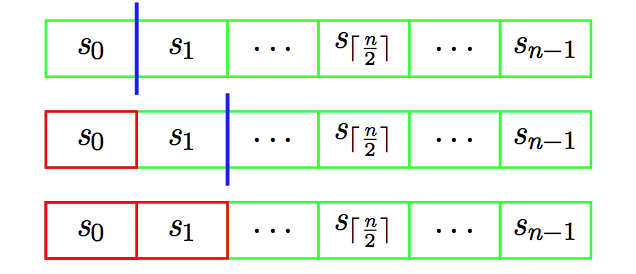
\includegraphics[width=2.5in]{L5-incremental-dc1.png}
%\end{figure}
%} 

%\frame{
%\frametitle{Properties of problems that greedy strategy can apply}
%
%\begin{enumerate}
% \item Divide-and-conquer: problem can be reduced into \textcolor{red}{\bf smaller, independent subproblems}; 
%
% \item {\bf Optimal substructure property}: an \textcolor{red}{\bf optimal solution} to the problem contains within it \textcolor{red}{optimal solutions} to subproblems. Thus we have a recursive solution as results. 
%
%\item {\bf Greedy selection property}: prove that at any stage, one of the locally-optimal choices can be used to construct the globally-optimal solution. 
%% 
%% \item top-down fashion: show that all but one subproblems induced by having made the greedy choice are empty. 
%\end{enumerate}
%}

%\frame{
%\begin{block}{}
% Revisiting {\sc Knapsack} problem
%\end{block}
%}

%\frame[allowframebreaks]{
%\frametitle{  {\sc Knapsack} problem}
%\begin{block}{}
%\begin{itemize}
%    \item {\bf Input:}\\ $n$ items. Item $i$ has weight $w_i$ and value $v_i$, and a total weight limit $W$; 
%	\item {\bf Output:}\\ A set of items to maximize the total value with total weight below $W$.
%\end{itemize}
% %\begin{itemize}
% %\item {\bf Input:} \\a set of items $i$ with weight $w$_$i$ and value $v$_$i$, and a total weight limit $W$, $i$=1,2,\cdots,$n$
% %\item {\bf Output:}\\the set of items which maximize the total value with total weight below $W$
% %\end{itemize}
%\end{block}
%Two versions of {\sc Knapsack } problem: 
%\begin{itemize}
% \item 
%{\sc 0-1 Knapsack}: each item, say gold ingot,  must be either taken or abandoned ;  \\
% \item
%{\sc Fractional Knapsack}: can take fractions of items, say gold dust. \\
%\end{itemize}
%	\begin{figure}
%	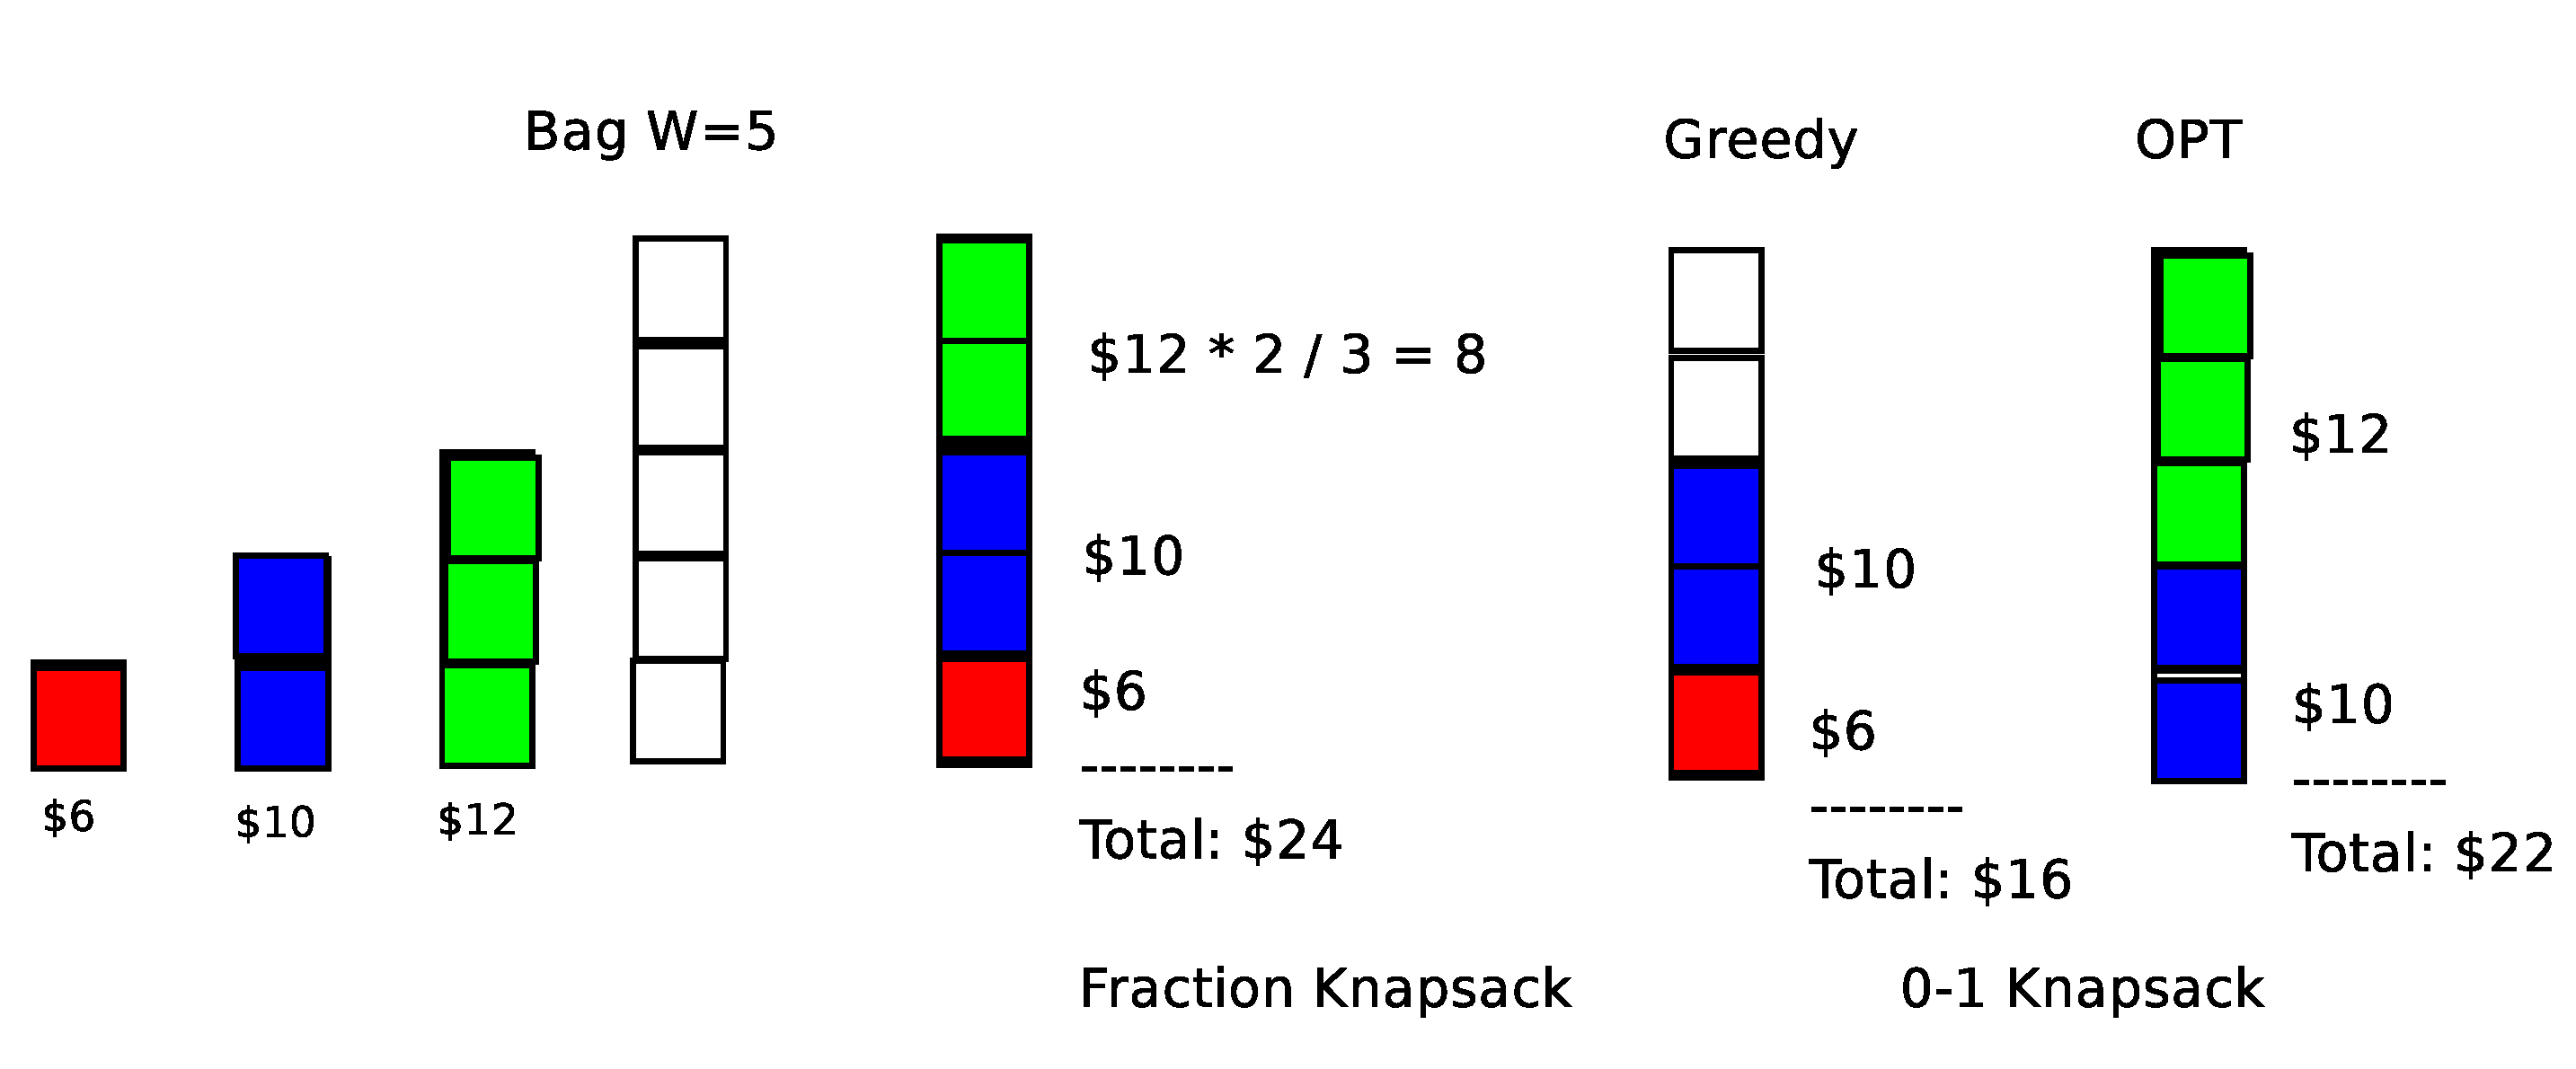
\includegraphics[width=3.5in]{L7-Knapsackexample.eps}
%	\end{figure}
%
%\begin{enumerate}
% \item Optimal substructure: both problems display the optimal substructure property; 
% \item Greedy choice property: however, the greedy choice property doesn't hold in the case of {\sc 0-1 Knapsack}--- the greedy choice of item 1 leads to a suboptimal solution. 
%\end{enumerate}
%}

\frame{
\begin{block}{}
 Revisiting {\sc ShortestPath} problem
\end{block}
%\footnote{Some pictures were excerpted from {\it Introduction to algorithms} }
}

\frame{
\frametitle{ Revisiting {\sc Single Source Shortest Paths} problem }

\begin{block}{}
 {\bf INPUT: } \\ 
A directed graph $G=<V, E>$. Each edge $e=<i, j>$ has a distance  $d_{i,j}$. A single source node $s$, and a destination node $t$; \\
 {\bf OUTPUT: } \\ 
The shortest path from $s$ to $t$.  \\
\end{block}

Two versions of {\sc ShortestPath} problem: \\
\begin{enumerate}
 \item No negative cycle: Bellman-Ford dynamic programming algorithm;
 \item No negative edge: Dijkstra greedy algorithm.
\end{enumerate}

% \begin{figure}
% 	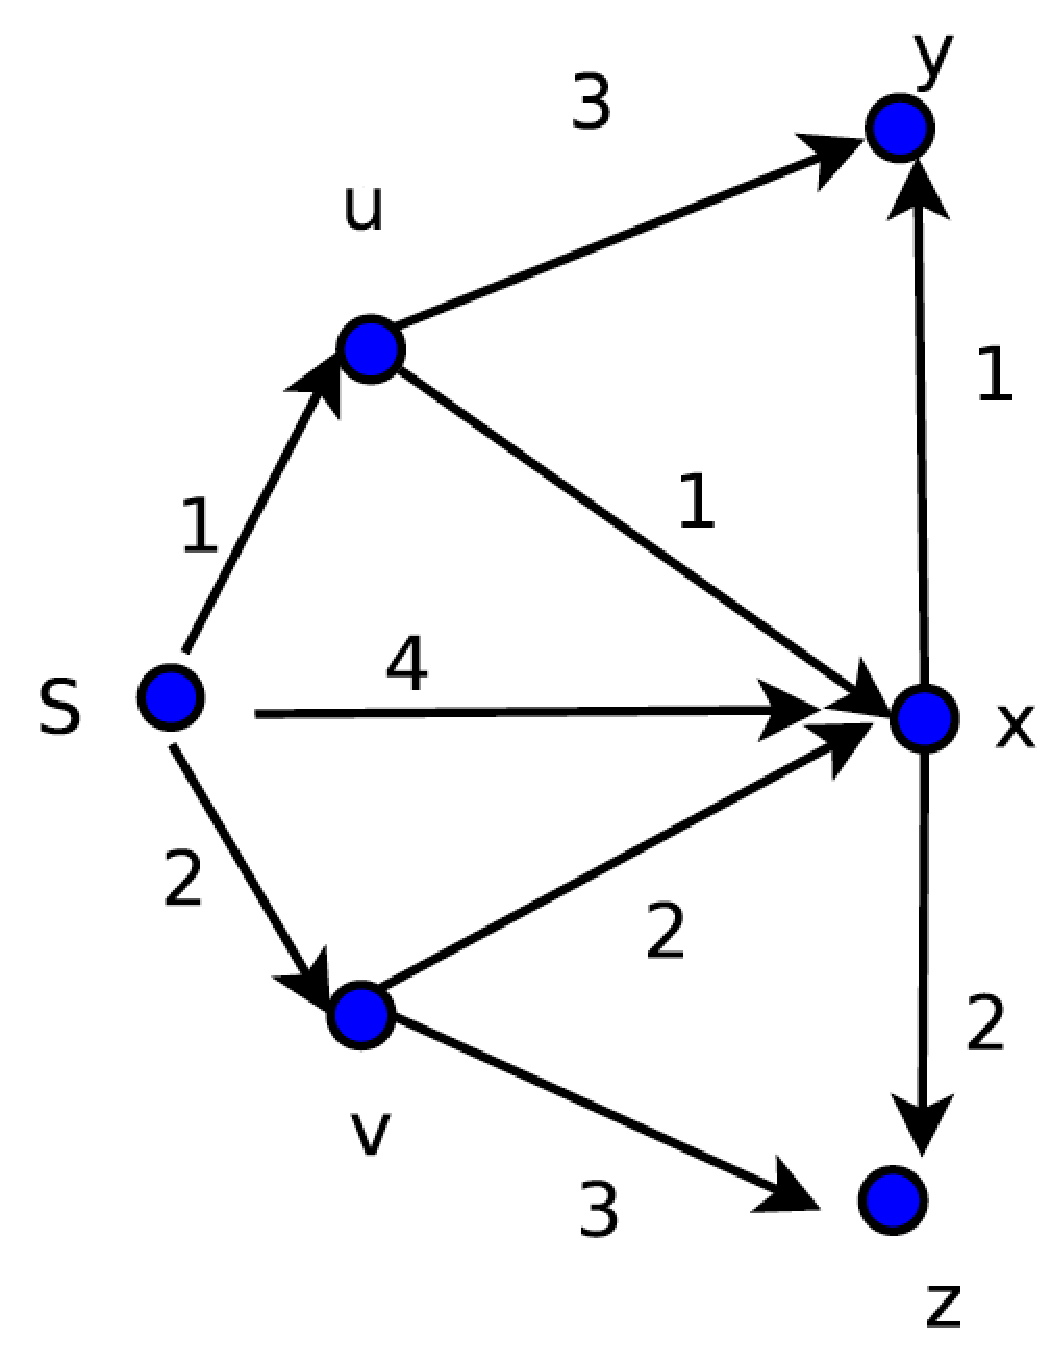
\includegraphics[width=2in]{L7-shortestpathexample.eps}
% \end{figure}
}


\frame{
	\begin{block}{}
	Optimal sub-structure property in version 1 
	\end{block} 
}

\frame{
\frametitle{Optimal sub-structure property }
\begin{itemize}
 \item Solution: a path from $s$ to $t$ with at most $(n-1)$ edges. Imagine the solving process as making a series of decisions; at each decision step, we decide the subsequent node. 
 \item Suppose we have already obtained an optimal solution $O$. Consider the final decision (i.e. from which we reach node $t$)  within $O$. There are several possibilities for the decision: 
  \begin{itemize}
   \item node $v$ such that $<v,t>\in E$: then it suffices to solve a smaller subproblem, i.e.  ``starting from $s$ to node $v$ via at most $(n-2)$ edges''. 
  \end{itemize}
 \item Thus we can design the general form of sub-problems as \textcolor{red}{\bf ``starting from $s$ to a node $v$ via at most $k$ edges''}. Denote the optimal solution value as $OPT(v, k)$. 
 \item Optimal substructure: 
\begin{footnotesize}
 $OPT(v, k) = \min \begin{cases} 
                      OPT( v, k-1 ) \\
                      \textcolor{blue}{\min_{<u,v>\in E}} \{ OPT( u, k-1) + d_{u, v}  \} \\
                     \end{cases}  $
\end{footnotesize}
\item Note: the first item $OPT(v, k-1)$ is introduced here to describe \textcolor{red}{\bf ``at most''}. 
\item Time complexity: $O(mn)$
\end{itemize}
} 


\frame{
\frametitle{ Bellman-Ford algorithm 1956 }

{\sc Bellman\_Ford}$( G, s, t )$
\begin{algorithmic}[1]
\FOR {$i=0$ to $n$ }
\STATE $OPT[s, i] = 0;$
\ENDFOR
\FOR{ any node $v \in V$ }
\STATE $OPT[v, 0] = \infty;$
\ENDFOR 
\FOR{ $k=1$ to $n-1$ }
\FORALL{ node $v$ (in an arbitrary order) }
\STATE \begin{small} $OPT[v, k] = \min \begin{cases}
		OPT[v, k-1], \\
		\min_{<u,v>\in E} \{OPT[ u, k-1 ] + d(u,v) \} 
		\end{cases}$
		\end{small}
\ENDFOR
\ENDFOR
\RETURN{ $OPT[ t, n-1]$};
\end{algorithmic}
}


\frame{
\frametitle{ An example  } 

\begin{figure}
 \begin{minipage}{0.40\textwidth}
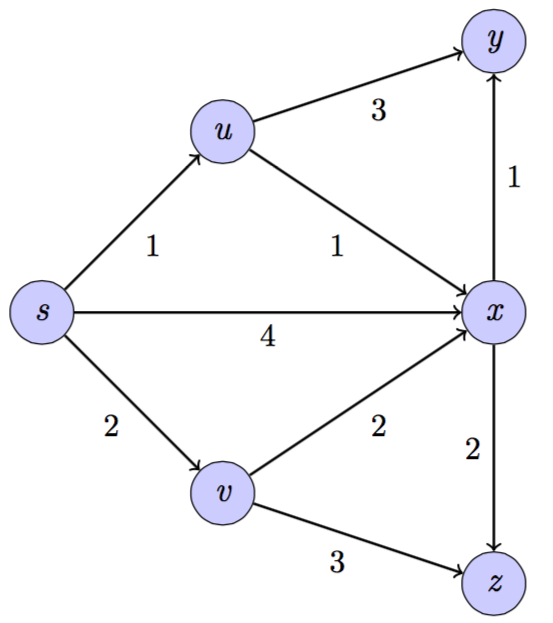
\includegraphics[width=\textwidth]{L7-shortestpathexample.png}

%\begin{tikzpicture}[auto,swap]
%
% 
%    \foreach \pos/\name in {{(0,0)/s}, {(2,2)/u}, {(2,-2)/v}, {(5,0)/x}, {(5,-3)/z}, {(5,3)/y}}
%        \node[vertex,fill=blue!20] (\name) at \pos {$\name$};
%        
%        
%    \foreach \source/\dest/\weight in {s/u/1, s/v/2, s/x/4,   u/y/3,  u/x/1, x/y/1, v/x/2, v/z/3, x/z/2 } 
%            \path[edge] (\source) -- node[weight] {$\weight$} (\dest);
%	
%\end{tikzpicture} 
				
 
 \end{minipage}
 \begin{minipage}{0.45\textwidth}

%  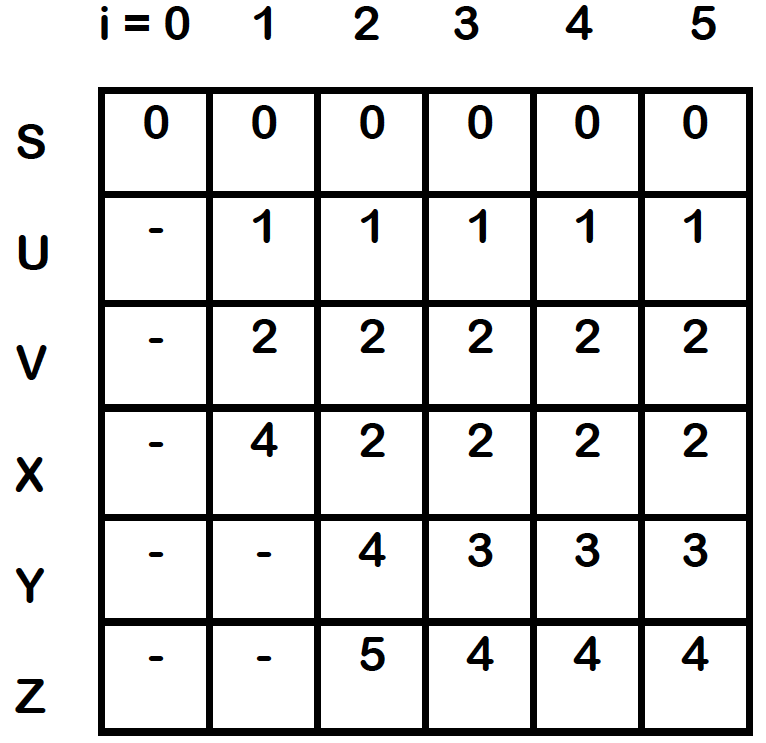
\includegraphics[width=\textwidth]{L7-Dijkstraexample.png}
 
 \begin{tikzpicture}[auto,swap]
  
  	\def\d{0.7};
	
	%draw index 
 \def\dy{1};
 \def\dx{0};

    \foreach \i/\num/\name in { 1/k=0/, 2/1/s1,3/2/s2,4/3/s3,5/4/s4,6/5/}{
           \node[blue,thick] (\name) at (\i*\d+\d/2 + \dx*\d - \d, \d/2 + \dy * \d) {\tt \num};
    }

 \def\dy{0};
 \def\dx{0};
    \foreach \i/\num/\name in { 1/S/s1,2/U/s2,3/V/s3,4/X/s4, 5/Y/,6/Z/}{
         \node[blue,thick] (\name) at ( -1*\d+\d/2,  0.0 - \i*\d + \d/2 - \dy * \d + \d){\tt  \num};
    }

    
%score	
 \def\dy{0};
 \def\dx{0};
    \foreach \i/\num/\name in { 0/0/,1/0/S1,2/0/S2,3/0/,4/0/,5/0/}{
             \draw[  thick ] (\i*\d + \dx*\d,  0+ \dy*\d) rectangle (\i*\d+\d + \dx*\d, \d + \dy*\d);
         \node (\name) at (\i*\d+\d/2 + \dx*\d, \d/2 + \dy*\d) {\tiny $\num$};
    }



%   \draw[blue,ultra thick] (S1) circle[radius=\d/2];
%   \draw[blue,ultra thick] (S2) circle[radius=\d/2];
%   \draw[blue,ultra thick] (L) circle[radius=\d/2];
%
    
        
 \def\dy{-1};
 \def\dx{0};
    \foreach \i/\num/\name in { 0/-/,1/1/S1,2/1/,3/1/S3,4/1/,5/1/}{
             \draw[  thick ] (\i*\d + \dx*\d,  0+ \dy*\d) rectangle (\i*\d+\d + \dx*\d, \d + \dy*\d);
         \node (\name) at (\i*\d+\d/2 + \dx*\d, \d/2 + \dy*\d) {\tiny $\num$};
    }
 
    %  \draw[red,ultra thick] (S1) circle[radius=\d/2];
   
    
 \def\dy{-2};
 \def\dx{0};
    \foreach \i/\num/\name in { 0/-/,1/2/,2/2/S1,3/2/S3,4/2/,5/2/}{
             \draw[  thick ] (\i*\d + \dx*\d,  0+ \dy*\d) rectangle (\i*\d+\d + \dx*\d, \d + \dy*\d);
         \node (\name) at (\i*\d+\d/2 + \dx*\d, \d/2 + \dy*\d) {\tiny $\num$};
    }
 
    
  \def\dy{-3};
 \def\dx{0};
    \foreach \i/\num/\name in { 0/-/,1/4/,2/2/S1,3/2/S3,4/2/,5/2/}{
             \draw[  thick ] (\i*\d + \dx*\d,  0+ \dy*\d) rectangle (\i*\d+\d + \dx*\d, \d + \dy*\d);
         \node (\name) at (\i*\d+\d/2 + \dx*\d, \d/2 + \dy*\d) {\tiny $\num$};
    }
   
  \def\dy{-4};
 \def\dx{0};
    \foreach \i/\num/\name in { 0/-/,1/-/,2/4/,3/3/S1,4/3/,5/3/}{
             \draw[  thick ] (\i*\d + \dx*\d,  0+ \dy*\d) rectangle (\i*\d+\d + \dx*\d, \d + \dy*\d);
         \node (\name) at (\i*\d+\d/2 + \dx*\d, \d/2 + \dy*\d) {\tiny $\num$};
    }

  \def\dy{-5};
 \def\dx{0};
    \foreach \i/\num/\name in { 0/-/,1/-/,2/5/,3/4/S3,4/4/S1,5/4/}{
             \draw[  thick ] (\i*\d + \dx*\d,  0+ \dy*\d) rectangle (\i*\d+\d + \dx*\d, \d + \dy*\d);
         \node (\name) at (\i*\d+\d/2 + \dx*\d, \d/2 + \dy*\d) {\tiny $\num$};
    }
 

\end{tikzpicture} 
 
 \end{minipage}
\end{figure}
}

\frame{
	\begin{block}{}
	Greedy-selection property in  version 2 
	\end{block} 
}

\frame{
\frametitle{ Greedy-selection property } 
% \begin{footnotesize}
%  $OPT(k, v) = \min \begin{cases} 
%                       OPT( k-1, v) \\
%                       \min_{<u,v>\in E} OPT( k-1, u) + d_{u,v}  \\
%                      \end{cases} $
% \end{footnotesize}

 \begin{itemize}
\item At the $k$-th step, let's consider a special node $v^*$, the nearest node from $s$ via at most $k-1$ edges, i.e. 
$OPT(  v^*, k-1 ) = min_v OPT( v, k-1 )$.  \\
\ \\
\  \\
\item Consider the optimal substructure property for $v^*$, i.e. 
\begin{small} 
 $OPT(v^*, k ) = \min \begin{cases} 
                      OPT(  v^*, k-1) \\
                      \min_{<u,v^*>\in E} \{ OPT( u, k-1 ) + d_{u, v^*} \}  \\
                     \end{cases} $
\end{small} 
\ \\
\ \\
\ \\
\item The above equality can be further simplified as: \\
 $OPT( v^*, k ) = OPT(  v^*, k-1 ) $ \\(Why? $OPT(  u, k-1 )\geq OPT(v^*, k-1)$ and $d_{u,v^*} \geq 0$.)  \\
\end{itemize}
}

\frame{
\frametitle{ The meaning of $OPT(v^*, k) = OPT( v^*, k-1) $ } 
\begin{figure}
 \begin{minipage}{0.40\textwidth}
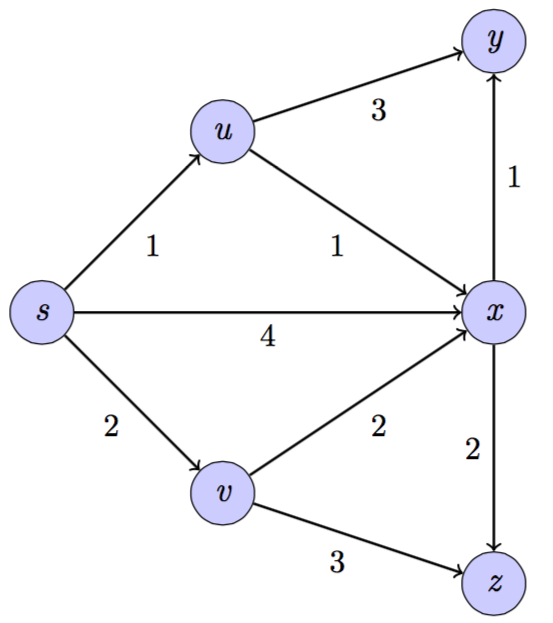
\includegraphics[width=0.9\textwidth]{L7-shortestpathexample.png}
 
%\begin{tikzpicture}[auto,swap]
% 
%    \foreach \pos/\name in {{(0,0)/s}, {(2,2)/u}, {(2,-2)/v}, {(5,0)/x}, {(5,-3)/z}, {(5,3)/y}}
%        \node[vertex,fill=blue!20] (\name) at \pos {$\name$};
%        
%        
%    \foreach \source/\dest/\weight in {s/u/1, s/v/2, s/x/4,   u/y/3,  u/x/1, x/y/1, v/x/2, v/z/3, x/z/2 } 
%            \path[edge] (\source) -- node[weight] {$\weight$} (\dest);
%	
%\end{tikzpicture} 
%		

 
 
 \end{minipage}
 \begin{minipage}{0.45\textwidth}

%  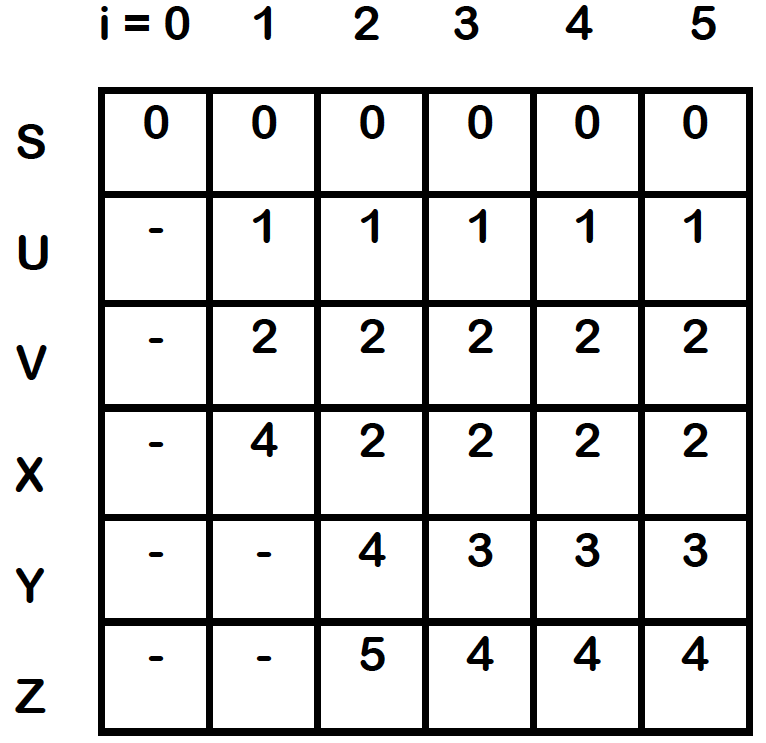
\includegraphics[width=\textwidth]{L7-Dijkstraexample.png}
 
 \begin{tikzpicture}[scale=0.8, auto,swap]
  
  	\def\d{0.7};
	
	%draw index 
 \def\dy{1};
 \def\dx{0};

    \foreach \i/\num/\name in { 1/k=0/, 2/1/s1,3/2/s2,4/3/s3,5/4/s4,6/5/}{
           \node[blue,thick] (\name) at (\i*\d+\d/2 + \dx*\d - \d, \d/2 + \dy * \d) {\tt \num};
    }

 \def\dy{0};
 \def\dx{0};
    \foreach \i/\num/\name in { 1/S/s1,2/U/s2,3/V/s3,4/X/s4, 5/Y/,6/Z/}{
         \node[blue,thick] (\name) at ( -1*\d+\d/2,  0.0 - \i*\d + \d/2 - \dy * \d + \d){\tt  \num};
    }

    
%score	
 \def\dy{0};
 \def\dx{0};
    \foreach \i/\num/\name in { 0/0/,1/0/S1,2/0/S2,3/0/,4/0/,5/0/}{
             \draw[  thick ] (\i*\d + \dx*\d,  0+ \dy*\d) rectangle (\i*\d+\d + \dx*\d, \d + \dy*\d);
         \node (\name) at (\i*\d+\d/2 + \dx*\d, \d/2 + \dy*\d) {\tiny $\num$};
    }



%   \draw[blue,ultra thick] (S1) circle[radius=\d/2];
%   \draw[blue,ultra thick] (S2) circle[radius=\d/2];
%   \draw[blue,ultra thick] (L) circle[radius=\d/2];
%
    
       
 \def\dy{-1};
 \def\dx{0};
    \foreach \i/\num/\name in { 0/-/,1/1/S1,2/1/,3/1/S3,4/1/,5/1/}{
             \draw[  thick ] (\i*\d + \dx*\d,  0+ \dy*\d) rectangle (\i*\d+\d + \dx*\d, \d + \dy*\d);
         \node (\name) at (\i*\d+\d/2 + \dx*\d, \d/2 + \dy*\d) {\tiny $\num$};
    }
 
      \draw[red,ultra thick] (S1) circle[radius=\d/2];
   
    
 \def\dy{-2};
 \def\dx{0};
    \foreach \i/\num/\name in { 0/-/,1/2/,2/2/S1,3/2/S3,4/2/,5/2/}{
             \draw[  thick ] (\i*\d + \dx*\d,  0+ \dy*\d) rectangle (\i*\d+\d + \dx*\d, \d + \dy*\d);
         \node (\name) at (\i*\d+\d/2 + \dx*\d, \d/2 + \dy*\d) {\tiny $\num$};
    }
       \draw[red,ultra thick] (S1) circle[radius=\d/2];
 
    
  \def\dy{-3};
 \def\dx{0};
    \foreach \i/\num/\name in { 0/-/,1/4/,2/2/S1,3/2/S3,4/2/,5/2/}{
             \draw[  thick ] (\i*\d + \dx*\d,  0+ \dy*\d) rectangle (\i*\d+\d + \dx*\d, \d + \dy*\d);
         \node (\name) at (\i*\d+\d/2 + \dx*\d, \d/2 + \dy*\d) {\tiny $\num$};
    }
       \draw[red,ultra thick] (S1) circle[radius=\d/2];
  
  \def\dy{-4};
 \def\dx{0};
    \foreach \i/\num/\name in { 0/-/,1/-/,2/4/,3/3/S1,4/3/,5/3/}{
             \draw[  thick ] (\i*\d + \dx*\d,  0+ \dy*\d) rectangle (\i*\d+\d + \dx*\d, \d + \dy*\d);
         \node (\name) at (\i*\d+\d/2 + \dx*\d, \d/2 + \dy*\d) {\tiny $\num$};
    }
         \draw[red,ultra thick] (S1) circle[radius=\d/2];

  \def\dy{-5};
 \def\dx{0};
    \foreach \i/\num/\name in { 0/-/,1/-/,2/5/,3/4/S3,4/4/S1,5/4/}{
             \draw[  thick ] (\i*\d + \dx*\d,  0+ \dy*\d) rectangle (\i*\d+\d + \dx*\d, \d + \dy*\d);
         \node (\name) at (\i*\d+\d/2 + \dx*\d, \d/2 + \dy*\d) {\tiny $\num$};
    }
        \draw[red,ultra thick] (S1) circle[radius=\d/2];
 


%draw blue rectangles 

 \def\dy{-1};
 \def\dx{0};
    \foreach \i/\num/\name in { 2/1/,3/1/S3,4/1/,5/1/}{
             \draw[  thick, green ] (\i*\d + \dx*\d,  0+ \dy*\d) rectangle (\i*\d+\d + \dx*\d, \d + \dy*\d);
    }
 
     
    
 \def\dy{-2};
 \def\dx{0};
    \foreach \i/\num/\name in { 3/2/S3,4/2/,5/2/}{
             \draw[  thick, green  ] (\i*\d + \dx*\d,  0+ \dy*\d) rectangle (\i*\d+\d + \dx*\d, \d + \dy*\d);
      }
 
    
  \def\dy{-3};
 \def\dx{0};
    \foreach \i/\num/\name in { 3/2/S3,4/2/,5/2/}{
             \draw[  thick, green ] (\i*\d + \dx*\d,  0+ \dy*\d) rectangle (\i*\d+\d + \dx*\d, \d + \dy*\d);
    }
 
   \def\dy{-4};
 \def\dx{0};
    \foreach \i/\num/\name in { 4/3/,5/3/}{
             \draw[  thick, green ] (\i*\d + \dx*\d,  0+ \dy*\d) rectangle (\i*\d+\d + \dx*\d, \d + \dy*\d);
    }
 
  \def\dy{-5};
 \def\dx{0};
    \foreach \i/\num/\name in {5/4/}{
             \draw[  thick, green ] (\i*\d + \dx*\d,  0+ \dy*\d) rectangle (\i*\d+\d + \dx*\d, \d + \dy*\d);
     }

\end{tikzpicture} 
 
 \end{minipage}
\end{figure}

\begin{enumerate}
\item  Intuitively $v^*$ (in red circles) can be treated as \textcolor{red}{\bf has already been explored using at most $(k-1)$ edges}, and the distance will not change afterwards.
\item  Thus, the calculations of $OPT(v^*, k)$ (in green rectangles) are in fact redundant.
\item In other words, it suffices to calculate $OPT( v, k) = \min_{<u,v>\in E} \{ OPT( u, k-1) + d_{u,v} \}$ for the \textcolor{red}{\bf unexplored nodes} $v \neq v^*$.
\end{enumerate}
}

\frame{
	\begin{block}{}
	But how to calculate $OPT( v, k )$ for the \textcolor{red}{\bf unexplored nodes} $v \notin S$? \\
	Let's see a greedy selection rule. 
	\end{block}
}

\frame{
%\frametitle{ Greedy selection property} 
\begin{footnotesize}
\begin{Theorem}
Let $S$ denote the \textcolor{blue}{\bf explored} nodes. \textcolor{red}{\bf Consider the nearest unexplored node $u^*$}, i.e., $u^*$ is the node $u$ ($u \notin S$) that minimizes $d'(u)=\min_{w\in S}\{d(w)+d(w, u)\}$. Then the path $P=s\rightarrow...\rightarrow w \rightarrow u^*$  is one of the shortest paths from $s$ to $u^*$ with distance $d'(u^*)$. 
\end{Theorem}
\begin{Proof} 
\begin{itemize}
\begin{footnotesize}
 \item Suppose there is another path $P'$ from $s$ to $u^*$ shorter than $P$. 
 \item Without loss of generality, we denote $P'= s \rightarrow...\rightarrow x \rightarrow y \rightarrow...\rightarrow u^*$. Here, $y$ denotes the first node in $P'$ leaving out of $S$. 
 \item 
 But $ |P'|  \geq   d(s, x) + d(x, y)    \geq   d'(u^*)$. A contradiction. 
%\begin{figure}
%	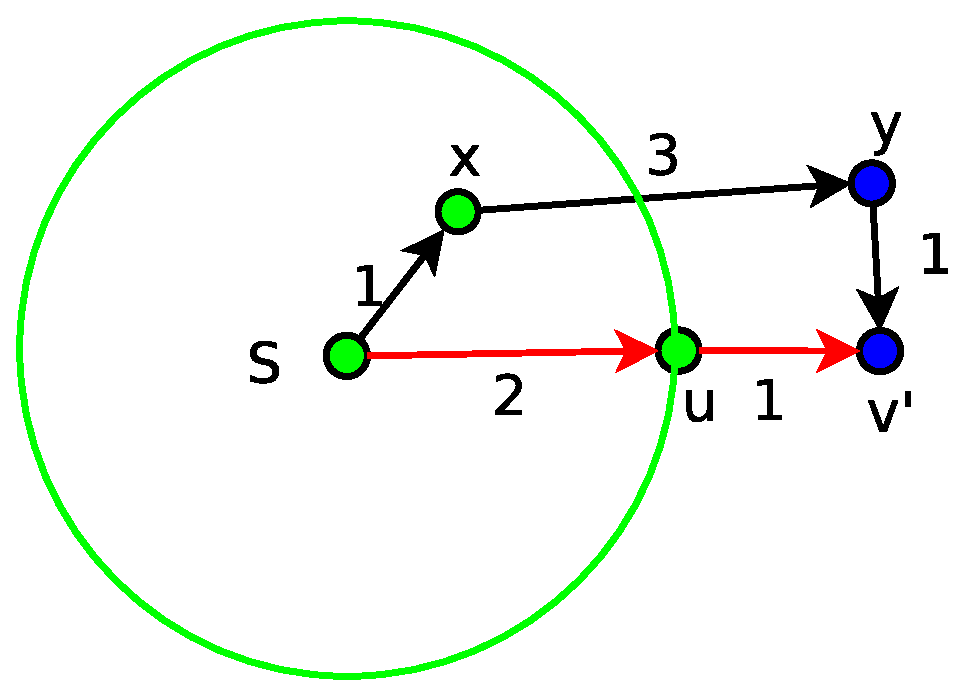
\includegraphics[width=1.5in]{L7-Dijkstraalgoalgoproof.eps}
%\end{figure}
\begin{figure}
\begin{tikzpicture}[scale=0.9, auto,swap]
 
   \draw[fill=gray!20, draw=white] (0,0) circle[radius=2];

    \foreach \pos/\name in {{(0,0)/s}, {(2,0)/w}, {(0, 1)/x}, {(3,1)/y}, {(3,0)/u^*}}
        \node[middlevertex,fill=blue!20] (\name) at \pos {$\name$};
        
        
    \foreach \source/\dest/\weight in {s/w/2, s/x/1, x/y/3,   y/u^*/1, w/u^*/1 } 
            \path[edge] (\source) -- node{\small $\weight$} (\dest);

        
    \foreach \source/\dest/\weight in {s/w/2,  w/u^*/1 } 
            \path[edge, red] (\source) -- node{\small $\weight$} (\dest);

   \node[red, ultra thick] at (0,-1) {$S: $ explored area}; 	
		
\end{tikzpicture} 
\end{figure}   
\end{footnotesize}
\end{itemize}
\end{Proof}
\end{footnotesize}
}


\frame{
	\frametitle{Key observations} 
	\begin{enumerate}
		\item  {\footnotesize Let $v^*$ denote the nearest node from  $s$ using at most $k-1$ edges.  The shortest distance $d(v^*)$ will not change afterwards. } 

\begin{figure}
 \begin{minipage}{0.40\textwidth}
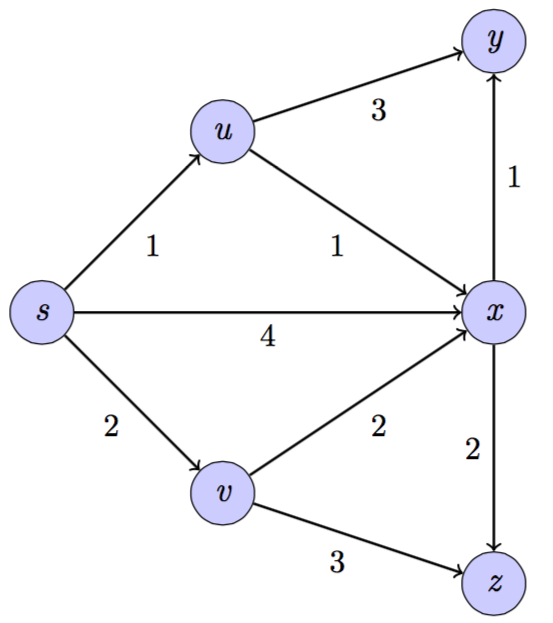
\includegraphics[width=0.8\textwidth]{L7-shortestpathexample.png}
 
%\begin{tikzpicture}[auto,swap]
% 
%    \foreach \pos/\name in {{(0,0)/s}, {(2,2)/u}, {(2,-2)/v}, {(5,0)/x}, {(5,-3)/z}, {(5,3)/y}}
%        \node[vertex,fill=blue!20] (\name) at \pos {$\name$};
%        
%        
%    \foreach \source/\dest/\weight in {s/u/1, s/v/2, s/x/4,   u/y/3,  u/x/1, x/y/1, v/x/2, v/z/3, x/z/2 } 
%            \path[edge] (\source) -- node[weight] {$\weight$} (\dest);
%	
%\end{tikzpicture} 
%		

 
 
 \end{minipage}
 \begin{minipage}{0.45\textwidth}

%  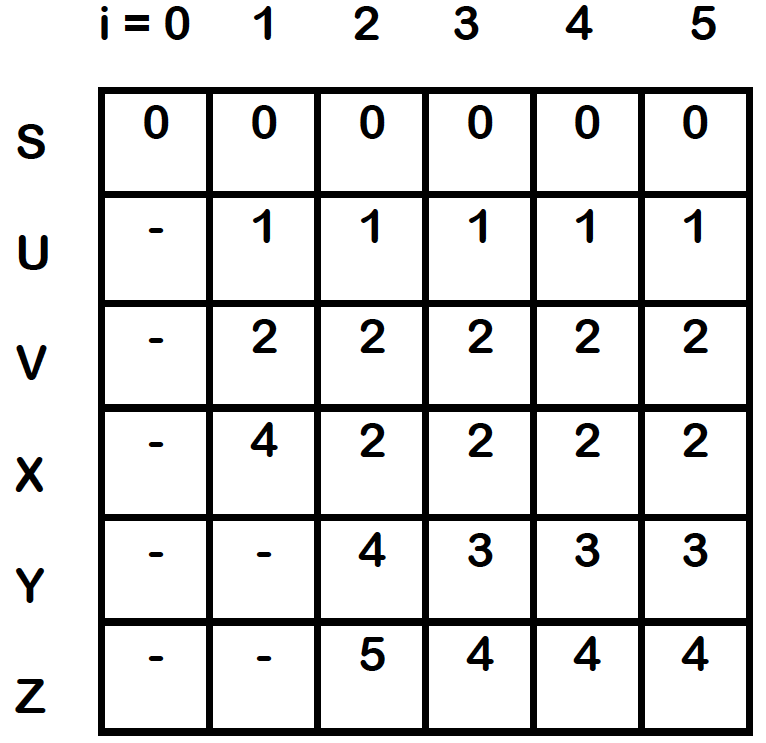
\includegraphics[width=\textwidth]{L7-Dijkstraexample.png}
 
 \begin{tikzpicture}[scale=0.7, auto,swap]
  
  	\def\d{0.7};
	
	%draw index 
 \def\dy{1};
 \def\dx{0};

    \foreach \i/\num/\name in { 1/k=0/, 2/1/s1,3/2/s2,4/3/s3,5/4/s4,6/5/}{
           \node[blue,thick] (\name) at (\i*\d+\d/2 + \dx*\d - \d, \d/2 + \dy * \d) {\tt \num};
    }

 \def\dy{0};
 \def\dx{0};
    \foreach \i/\num/\name in { 1/S/s1,2/U/s2,3/V/s3,4/X/s4, 5/Y/,6/Z/}{
         \node[blue,thick] (\name) at ( -1*\d+\d/2,  0.0 - \i*\d + \d/2 - \dy * \d + \d){\tt  \num};
    }

    
%score	
 \def\dy{0};
 \def\dx{0};
    \foreach \i/\num/\name in { 0/0/,1/0/S1,2/0/S2,3/0/,4/0/,5/0/}{
             \draw[  thick ] (\i*\d + \dx*\d,  0+ \dy*\d) rectangle (\i*\d+\d + \dx*\d, \d + \dy*\d);
         \node (\name) at (\i*\d+\d/2 + \dx*\d, \d/2 + \dy*\d) {\tiny $\num$};
    }



%   \draw[blue,ultra thick] (S1) circle[radius=\d/2];
%   \draw[blue,ultra thick] (S2) circle[radius=\d/2];
%   \draw[blue,ultra thick] (L) circle[radius=\d/2];
%
    
       
 \def\dy{-1};
 \def\dx{0};
    \foreach \i/\num/\name in { 0/-/,1/1/S1,2/1/,3/1/S3,4/1/,5/1/}{
             \draw[  thick ] (\i*\d + \dx*\d,  0+ \dy*\d) rectangle (\i*\d+\d + \dx*\d, \d + \dy*\d);
         \node (\name) at (\i*\d+\d/2 + \dx*\d, \d/2 + \dy*\d) {\tiny $\num$};
    }
 
      \draw[red,ultra thick] (S1) circle[radius=\d/2];
   
    
 \def\dy{-2};
 \def\dx{0};
    \foreach \i/\num/\name in { 0/-/,1/2/,2/2/S1,3/2/S3,4/2/,5/2/}{
             \draw[  thick ] (\i*\d + \dx*\d,  0+ \dy*\d) rectangle (\i*\d+\d + \dx*\d, \d + \dy*\d);
         \node (\name) at (\i*\d+\d/2 + \dx*\d, \d/2 + \dy*\d) {\tiny $\num$};
    }
       \draw[red,ultra thick] (S1) circle[radius=\d/2];
 
    
  \def\dy{-3};
 \def\dx{0};
    \foreach \i/\num/\name in { 0/-/,1/4/,2/2/S1,3/2/S3,4/2/,5/2/}{
             \draw[  thick ] (\i*\d + \dx*\d,  0+ \dy*\d) rectangle (\i*\d+\d + \dx*\d, \d + \dy*\d);
         \node (\name) at (\i*\d+\d/2 + \dx*\d, \d/2 + \dy*\d) {\tiny $\num$};
    }
       \draw[red,ultra thick] (S1) circle[radius=\d/2];
  
  \def\dy{-4};
 \def\dx{0};
    \foreach \i/\num/\name in { 0/-/,1/-/,2/4/,3/3/S1,4/3/,5/3/}{
             \draw[  thick ] (\i*\d + \dx*\d,  0+ \dy*\d) rectangle (\i*\d+\d + \dx*\d, \d + \dy*\d);
         \node (\name) at (\i*\d+\d/2 + \dx*\d, \d/2 + \dy*\d) {\tiny $\num$};
    }
         \draw[red,ultra thick] (S1) circle[radius=\d/2];

  \def\dy{-5};
 \def\dx{0};
    \foreach \i/\num/\name in { 0/-/,1/-/,2/5/,3/4/S3,4/4/S1,5/4/}{
             \draw[  thick ] (\i*\d + \dx*\d,  0+ \dy*\d) rectangle (\i*\d+\d + \dx*\d, \d + \dy*\d);
         \node (\name) at (\i*\d+\d/2 + \dx*\d, \d/2 + \dy*\d) {\tiny $\num$};
    }
        \draw[red,ultra thick] (S1) circle[radius=\d/2];
 


%draw blue rectangles 

 \def\dy{-1};
 \def\dx{0};
    \foreach \i/\num/\name in { 2/1/,3/1/S3,4/1/,5/1/}{
             \draw[  thick, green ] (\i*\d + \dx*\d,  0+ \dy*\d) rectangle (\i*\d+\d + \dx*\d, \d + \dy*\d);
    }
 
     
    
 \def\dy{-2};
 \def\dx{0};
    \foreach \i/\num/\name in { 3/2/S3,4/2/,5/2/}{
             \draw[  thick, green  ] (\i*\d + \dx*\d,  0+ \dy*\d) rectangle (\i*\d+\d + \dx*\d, \d + \dy*\d);
      }
 
    
  \def\dy{-3};
 \def\dx{0};
    \foreach \i/\num/\name in { 3/2/S3,4/2/,5/2/}{
             \draw[  thick, green ] (\i*\d + \dx*\d,  0+ \dy*\d) rectangle (\i*\d+\d + \dx*\d, \d + \dy*\d);
    }
 
   \def\dy{-4};
 \def\dx{0};
    \foreach \i/\num/\name in { 4/3/,5/3/}{
             \draw[  thick, green ] (\i*\d + \dx*\d,  0+ \dy*\d) rectangle (\i*\d+\d + \dx*\d, \d + \dy*\d);
    }
 
  \def\dy{-5};
 \def\dx{0};
    \foreach \i/\num/\name in {5/4/}{
             \draw[  thick, green ] (\i*\d + \dx*\d,  0+ \dy*\d) rectangle (\i*\d+\d + \dx*\d, \d + \dy*\d);
     }

\end{tikzpicture} 
 
 \end{minipage}
\end{figure}


		
		\item {\footnotesize Let's $u^*$ denote the nearest unexplored node. The shortest distance can be determined.  }
\begin{figure}
\begin{tikzpicture}[scale=0.9, auto,swap]
 
   \draw[fill=gray!20, draw=white] (0,0) circle[radius=2];

    \foreach \pos/\name in {{(0,0)/s}, {(2,0)/w}, {(0, 1)/x}, {(3,1)/y}, {(3,0)/u^*}}
        \node[middlevertex,fill=blue!20] (\name) at \pos {$\name$};
        
        
    \foreach \source/\dest/\weight in {s/w/2, s/x/1, x/y/3,   y/u^*/1, w/u^*/1 } 
            \path[edge] (\source) -- node{\small $\weight$} (\dest);

        
    \foreach \source/\dest/\weight in {s/w/2,  w/u^*/1 } 
            \path[edge, red] (\source) -- node{\small $\weight$} (\dest);

   \node[red, ultra thick] at (0,-1) {$S: $ explored area}; 	
		
\end{tikzpicture} 
\end{figure}   

	\end{enumerate}

}

\frame{
\frametitle{ Dijkstra's algorithm [1959] }
\begin{small}
{\sc Dijkstra}$(G, s )$
\begin{algorithmic}[1]
\STATE $S=\{s\}$; //$S$ denotes the set of explored nodes,
\STATE $d(s)=0$; //$d(u)$ stores an upper bound of the shortest-path weight from $s$ to $u$;
\FORALL{ node $v \neq s$}
\STATE{ $d(v) = +\infty$; } 
\ENDFOR
\WHILE{$S \neq V$}
\FORALL{ node $v \notin S$}
\STATE  $d(v)=\min_{u\in S}\{d(u)+d(u,v)\}$;
\ENDFOR 
\STATE \textcolor{red}{Select the node $v^*$ ($v^* \notin S$) that minimizes} $d(v)$;
\STATE $S=S \cup \{v^*\}$;
\ENDWHILE
\end{algorithmic}
\end{small} 
\begin{itemize}
\item 
Line $(8-10)$ is called {\bf "relaxing"}. That is, we test whether the shortest-path to $v$ found so far can be improved by going through $u$, and if so, update $d(v)$. 
\item In the case that $d_{u,v} = 1$ for any $u,v$ pair, Dijkstra's algorithm 
reduces to BFS. Thus, Dijkstra's algorithm can be treated as a weighted version of BFS. 
\end{itemize}

}








\frame{
\frametitle{ Implementing Dijkstra algorithm using priority queue }


\begin{small}
{\sc Dijkstra}$( G, s )$
\begin{algorithmic}[1]
\STATE $key(s) = 0;$  //$key(u)$ stores an upper bound of the shortest-path weight from $s$ to $u$;
\STATE $PQ.$ {\sc Insert} $(s)$;
\STATE $S=\{ s \}$; // Let $S$ be the set of explored nodes;
\FORALL{ node $v \neq s$ }
\STATE $key(v) = +\infty $
\STATE $PQ.$ {\sc Insert} $(v)$ \textcolor{red}{// n times}
\ENDFOR
\WHILE{$ S \neq V $}
\STATE $v=PQ.$ {\sc ExtractMin}$()$; \textcolor{red}{// n times}
\STATE $S=S \cup \{v\}$;
\FOR{ each $w \notin S$ and $<v, w> \in E$}
\IF{ $key(v) + d(v, w) < key(w)$}
\STATE $PQ.${\sc DecreaseKey}($w, key(v) + d(v, w)$); \textcolor{red}{// m times}
\ENDIF
\ENDFOR
\ENDWHILE
\end{algorithmic}
\end{small}
Here $PQ$ denotes a min-priority queue. 
(see a demo)
}





\frame{
\frametitle{ Contributions by Edsger W.  Dijkstra  }

\begin{figure}
 	 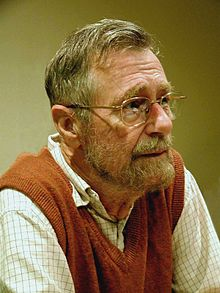
\includegraphics[width=1.1in]{Dijkstra.jpg}
\end{figure}
\begin{small} 
\begin{itemize} 
\item  The semaphore construct for coordinating multiple processors and programs. 
\item The concept  of self-stabilization – an alternative way to ensure the reliability of the system
\item  "A Case against the GO TO Statement", regarded as a major step towards the widespread deprecation of the GOTO statement and its effective replacement by structured control constructs, such as the while loop.
\item ...
\end{itemize}
\end{small} 
} 


\frame{
\frametitle{ {\sc ShortestPath}: Bellman-Ford algorithm vs. Dijkstra algorithm } 
A slight change of edge weights leads to a significant change of algorithm design. 
\begin{enumerate}
\item No negative cycle: an optimal path from $s$ to $v$ has at most $n-1$ edges; thus the optimal solution is $OPT( v, n-1)$. To calculate $OPT(v, n-1 )$, we appeal to the following recursion: 

$OPT[v, k] = \min \begin{cases}
		OPT[ v, k-1], \\
		\min_{<u,v>\in E} \{OPT[u, k-1 ] + d(u,v) \} 
		\end{cases}$
\ \\		
\item No negative edge: This stronger constraint on edge weights implies greedy choice property. In particular, it is not necessary to calculate $OPT(v, i)$ for any explored node $v \in S$, and for the nearest unexplored node, its shortest distance from $s$ is determined. 
\end{enumerate}
} 


\frame{
 	\begin{block}{}
	Time complexity analysis
	\end{block} 
} 

\frame{
	\frametitle{ Time complexity of {\sc Dijkstra} algorithm} 

  \begin{table}
  \begin{tabular}{crrrr}
  \hline  \hline
  Operation & Linked  & Binary  & Binomial  & Fibonacci  \\
            &  list &  heap &  heap & heap \\
  \hline
  {\sc MakeHeap} & $ 1 $ &  $1$  & $ 1 $ & $1$  \\ 
  {\sc Insert} & $ 1 $ &  $\log n$  & $ \log n $ & $1$  \\ 
   {\sc ExtractMin} & $ n $ &  $\log n$  & $ \log n  $ & $ \log n $  \\ 
  {\sc DecreaseKey} & $ 1 $ &  $\log n$  & $ \log n $ & $1$  \\ 
  {\sc Delete} & $ n $ &  $\log n$  & $ \log n $ & $\log n$  \\ 
  {\sc Union} & $ 1 $ &  $ n $  & $ \log n $ & $1$  \\ 
   {\sc FindMin} & $ n $ &  $1$  & $ \log n $ & $1$  \\ 
  \hline 
  {\sc Dijkstra} & $ O(n^2) $ &  $ O(m \log n) $  & $ O( m \log n ) $ & $ O( m + n \log n) $  \\ 
  \hline \hline 
  \end{tabular} 
  \end{table}
{\sc Dijkstra} algorithm: $n$ {\sc Insert}, $n$ {\sc ExtractMin}, and $m$ {\sc DecreaseKey}. 
}

\frame{
	\begin{block}{}
		Extension: can we reweigh the edges to make all weight positive?  
	\end{block}
}

\frame{
	\frametitle{Trial 1: increasing all edge weights  by the same amount } 

\begin{figure}
\begin{tikzpicture}[scale=1., auto,swap]
    % Draw a 7,11 network
    % First we draw the vertices
    \foreach \pos/\name/\label in {{(0,0)/s/s}, {(1.5,0)/u/u}, {(1,1)/v/v}, {(2,1)/w/w}, {(3, 0)/t/t}}
            \node[smallvertex,draw=black, fill=blue!20] (\name) at \pos {\tiny $\label$};
  
    % Connect vertices with edges and draw weights
  \foreach \source/ \dest /\weight in {s/u/{1}, s/v/{-1}, v/w/{1}, w/t/{-1}, u/t/{1}}
        \draw[->] (\source) -- node[weight,above] {\small $\weight$} (\dest);
%       \draw[dashed, ->] (0,0) arc  (120:60:2);

  \foreach \source/ \dest /\weight in {s/v/{-1}, v/w/{1}, w/t/{-1}}
        \draw[->, red] (\source) -- node[weight,above] {} (\dest);

\draw[->, green, ultra thick] (3.8, 0.5) -- (4.3, 0.5); 

   % Draw a 7,11 network
    % First we draw the vertices
    \foreach \pos/\name/\label in {{(5,0)/s/s}, {(6.5,0)/u/u}, {(6,1)/v/v}, {(7,1)/w/w}, {(8, 0)/t/t}}
            \node[smallvertex,draw=black, fill=blue!20] (\name) at \pos {\tiny $\label$};
  
    % Connect vertices with edges and draw weights
  \foreach \source/ \dest /\weight in {s/u/{6}, s/v/{4}, v/w/{6}, w/t/{4}, u/t/{6}}
        \draw[->] (\source) -- node[weight,above] {\small $\weight$} (\dest);
%       \draw[dashed, ->] (0,0) arc  (120:60:2);

  \foreach \source/ \dest /\weight in {s/u/{-1}, u/t/{-1}}
        \draw[->, red] (\source) -- node[weight,above] {} (\dest);


   \end{tikzpicture}
\end{figure}

\begin{itemize}
\item Increasing all the weight by 5 changes the shortest path from $s$ to $t$.
\item Reason: different paths might change by different amount although 	
all edges change by the same mount. 		
\end{itemize}

}

\frame{
	\frametitle{Trial 2: increasing an edge weight according to its two ends}
\begin{itemize}
\item Suppose each node $v$ is associated with a number $c(v)$. We reweigh an edge $(u, v)$ as follows.	
		$d'(u, v) = d( u, v) + c(u) - c(v)$ 	 
\item Note that  for any path $u \leadsto v$, we have 
		$d'(u \leadsto v) = d( u \leadsto v) + c(u) - c(v)$ 	 
\item  Advantage: the shortest path from $u$ to $v$ with the new weighting function is exact the same to that with the original weighting function. 
\item But how to define $c(v)$ to make all edge weight positive? 
\end{itemize}
} 

\frame{
	\frametitle{Reweighting schema} 
	\begin{itemize}
		\item Adding a new node $S$, and connect $S$ to each node $v$ with an edge weight $d( S, v) = 0$, $d( v, S) = \infty$
		\item Set $c(v)$ as $dist(S, v)$, the shortest distance from $S$ to $v$. 
		\item We can prove that for any node pair $u$ and $v$, 		 
			$d'(u, v) = d(u, v) + dist( u) - dist( v) \geq 0$. 
	\end{itemize}
}	

\frame{
	\frametitle{Johnson algorithm for all pairs shortest path [1977]}

\begin{small}
{\sc Johnson}$( G, d )$
\begin{algorithmic}[1]
\STATE Create a new node $s^*$; 
\FORALL{ node $v \neq s^*$} 
	\STATE{	$d(s^*, v) = 0$}
\ENDFOR
\STATE Run Bellman-Ford to calculate the shortest distance from $s^*$ to all nodes; 
\STATE Reweighting: 	$d'(u, v) = d(u, v) + dist( s^*, u) - dist(s^*, v) $ 
\FORALL{ node $u \neq s^*$} 
	\STATE Run Dijkstra's algorithm with the new weight $d'$ to calculate the shortest paths from $u$; 
	\FORALL{ node $v \neq s^*$}
		\STATE $dist( u, v) = dist(u, v)  - dist( s^*, u) + dist( s^*, v);$ 
	\ENDFOR
\ENDFOR 
\end{algorithmic}
\end{small}
Time complexity: $O( mn + n^2 \log n)$. 	
	
} 


\frame{
	\begin{block}{}
		Extension: data structures designed to speed up the Dijkstra's algorithm
	\end{block}
}

\frame{
\frametitle{Binary heap, Binomial heap, and Fibonacci heap} 

\begin{figure}
 \begin{minipage}{0.30\textwidth}
     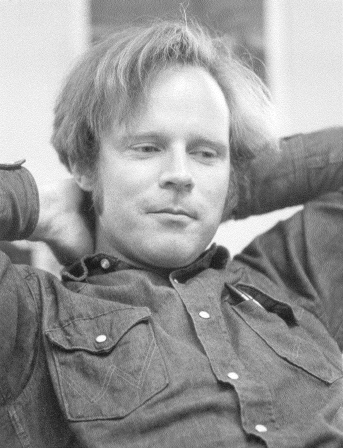
\includegraphics[width=0.8\textwidth]{Floyd.png}
 \end{minipage}
 \begin{minipage}{0.30\textwidth}
     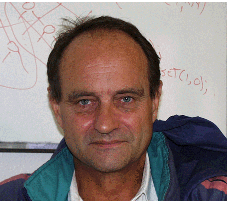
\includegraphics[width=0.8\textwidth]{JeanVuillemin.png}
 \end{minipage}
 \begin{minipage}{0.30\textwidth}
     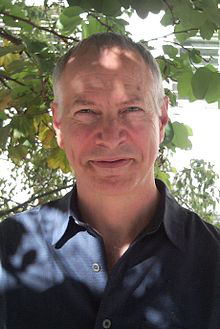
\includegraphics[width=0.8\textwidth]{Tarjan.png}
 \end{minipage}
 \caption{ Robert W. Floyd, Jean Vuillenmin, Robert Tarjan}
 \end{figure}

(See extra slides for binary heap, binomial heap and Fibonacci heap)
} 


\frame{
\begin{block}{}
 Matroid: theoretical foundation of greedy strategy
\end{block}
}

 \frame{
 \frametitle{ Revisiting  {\sc Maximal  Linearly Independent Set} problem}
\begin{itemize} 
\item Question:  Given a matrix, to determine the maximal linearly independent set. 
\item 
 Example: 
\begin{table}{
\begin{tabular}{lrrrrrrr}
$A_{1}=[$& 1 & 2 & 3 & 4 & 5 $]$   \\ 
$A_{2}=[$& 1 & 4 & 9 & 16 & 25 $]$   \\ 
$A_{3}=[$& 1 & 8 & 27 & 64 & 125 $]$  \\ 
$A_{4}=[$& 1 & 16 & 81 & 256 & 625 $]$  \\ 
$A_{5}=[$& 2 & 6 & 12 & 20 & 30 $]$  \\ 
\end{tabular}}{}
\end{table}
\item Independent vector set: $\{ A_1, A_2, A_3, A_4 \}$
\end{itemize}

} 

\frame{
\frametitle{ Calculating maximal number of independent vectors }

{\sc IndependentSet}$( M )$
\begin{algorithmic}[1]
\STATE $A=\{ \};$
\FORALL { row vector $v $  }
\IF { $A\cup\{v\}$ is still independent }
\STATE $A=A\cup\{v\}$;
\ENDIF
\ENDFOR
\RETURN $A$;
\end{algorithmic}
}

\frame{
	 \frametitle{ Correctness: Properties of linear independence vector set  }
Let's consider the {\bf linear independence} for vectors. 
 \begin{enumerate}
  \item \textcolor{red}{\bf Hereditary property:} if  $B$ is an  {\bf independent vector set}  and $A \subset B$, then $A $ is also an {\bf independent vector set} 
  \item \textcolor{red}{\bf Augmentation property:}  if both $A$  and $B$ are {\bf independent vector sets}, and $|A| < |B|$, then there is a vector $v \in B-A$ such that $A \cup \{v\}$ is still an {\bf independent vector set}  
 \end{enumerate}

Example: 
\begin{table}{
\begin{tabular}{lrrrrrrr}
$V_{1}=[$& 1 & 2 & 3 & 4 & 5 $]$   \\ 
$V_{2}=[$& 1 & 4 & 9 & 16 & 25 $]$   \\ 
$V_{3}=[$& 1 & 8 & 27 & 64 & 125 $]$  \\ 
$V_{4}=[$& 1 & 16 & 81 & 256 & 625 $]$  \\ 
$V_{5}=[$& 2 & 6 & 12 & 20 & 30 $]$  \\ 
\end{tabular}}{}
\end{table}
\begin{itemize} 
\item Independent vector sets: $A=\{ V_1, V_3, V_5 \}$, $B=\{ V_{1}, V_{2}, V_{3}, V_{4} \}$, and $|A| < |B|$. 
\item Augmentation of $A$: $A \cup \{V_{4} \}$ is also independent. 
\end{itemize}
}



\frame{
 \frametitle{  A weighted version }
\begin{itemize} 
\item Question:  Given a matrix, \textcolor{red}{\bf where each row vector is associated with a weight}, to determine a set of linearly independent vectors to maximize the sum of weight.  
\item 
 Example: 
\begin{table}{
\begin{tabular}{lrrrrrrl}
$A_{1}=[$& 1 & 2 & 3 & 4 & 5 $]$&\textcolor{red}{$W_{1}=9$} \\ 
$A_{2}=[$& 1 & 4 & 9 & 16 & 25 $]$&\textcolor{red}{$W_{2}=7$} \\ 
$A_{3}=[$& 1 & 8 & 27 & 64 & 125 $]$&\textcolor{red}{$W_{3}=5$}\\ 
$A_{4}=[$& 1 & 16 & 81 & 256 & 625 $]$&\textcolor{red}{$W_{4}=3$}\\ 
$A_{5}=[$& 2 & 6 & 12 & 20 & 30 $]$&\textcolor{red}{$W_{5}=1$}\\ 
\end{tabular}}{}
\end{table}
%\item Independent vector set: $\{ A_1, A_2, A_3, A_4 \}$
\end{itemize}

} 

\frame{
\frametitle{A general greedy algorithm  }

{\sc Matroid\_Greedy}$( M, W )$
\begin{algorithmic}[1]
\STATE $A=\{ \};$
\STATE \textcolor{red}{\bf Sort row vectors in the decreasing order of their weights;}
\FORALL { row vector $v $  }
\IF { $A\cup\{v\}$ is still independent }
\STATE $A=A\cup\{v\}$;
\ENDIF
\ENDFOR
\RETURN $A$;
\end{algorithmic}

Time complexity: $O(n\log n + n C(n) )$, where $C(n)$ is the time needed to check independence. 
}

\frame{
\frametitle{Matroid greedy algorithm:  correctness}

\begin{Theorem}{[Greedy-choice property]}
 Let $v$ be the vector with the largest weight and $\{v\}$ is independent, then there is an optimal vector set $A$ of $M$ and $A$ contains $v$. 
\end{Theorem}
%\begin{footnotesize}
\begin{Proof}
\begin{itemize}
 \item 
Assume there is an optimal subset $B$ but $v \notin B$; 
\item
We have
\item
Then we can construct $A$ from $B$ as follows: 
\begin{enumerate}
 \item 
Initially: $A=\{v\}$; \\
\item
Until $|A| = |B|$, repeatedly find a new element of $B$ that can be added to $A$ while preserving the independence of $A$ (by augmentation property);
\end{enumerate}
\item Finally we have $A=B-\{v'\} \cup \{v\}$.
\item We have $W(A) \geq W(B)$ since  $W(v) \geq W(v')$ for any $v' \in B$.  A contradiction.

\end{itemize}
\end{Proof}
%\end{footnotesize}

}


\frame{
\frametitle{Matroid greedy algorithm:  correctness cont'd}

\begin{Theorem}{[Optimal substructure property]}
 Let $v$ be the vector with the largest weight and $\{v\}$ is itself independent. The remaining problem reduces to finding an optimal subset in $M'$, where 
 $M'=\{ v' \in S,  \text{and }  v, v' \text{are independent} \}$
 \end{Theorem}
\begin{Proof} 
\begin{itemize}
\item Suppose $A'$ is an optimal independent set of $M'$.
\item Define $A=A' \cup \{ v \}$.
\item Then $A$ is also an independent set of $M$. 
\item And $A$ has the maximum weight $W(A) = W(A') + W(v)$. 
\end{itemize}
\end{Proof}
}

\frame{
\begin{block}{}
An extension of {\bf linear independence for vectors}: matroid
\end{block}
}


\frame{
 \frametitle{Matroid [Haussler Whitney, 1935] }
 \begin{figure}
	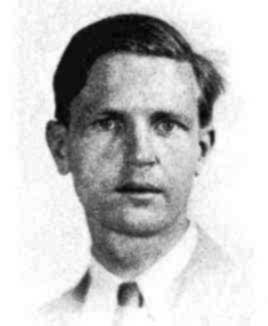
\includegraphics[width=1.25in]{Whitney.png}
\end{figure}
\begin{itemize}
	\item Matroid was proposed to capture the concept of \textcolor{red}{\bf linear independence} in matrix theory, and   generalize  the concept in other field, say \textcolor{red}{\bf graph theory}. 
	\item In fact, in the paper {\it On the abstract properties of linear independence},  Haussler Whitney said: 
	
	{\it 
	   This paper has a close connection with a paper by the author on linear graphs; we say a subgraph of a graph is \textcolor{red}{\bf independent} if it contains no circuit.
	}  
\end{itemize}

}



\frame{
	 \frametitle{ Origin 1 of matroid: linear independence for vectors  }
Let's consider the {\bf linear independence} for vectors. 
 \begin{enumerate}
  \item \textcolor{red}{\bf Hereditary property:} if  $B$ is an  {\bf independent vector set}  and $A \subset B$, then $A $ is also an {\bf independent vector set} 
  \item \textcolor{red}{\bf Augmentation property:}  if both $A$  and $B$ are {\bf independent vector sets}, and $|A| < |B|$, then there is a vector $v \in B-A$ such that $A \cup \{v\}$ is still an {\bf independent vector set}  
 \end{enumerate}

Example: 
\begin{table}{
\begin{tabular}{lrrrrrrr}
$V_{1}=[$& 1 & 2 & 3 & 4 & 5 $]$   \\ 
$V_{2}=[$& 1 & 4 & 9 & 16 & 25 $]$   \\ 
$V_{3}=[$& 1 & 8 & 27 & 64 & 125 $]$  \\ 
$V_{4}=[$& 1 & 16 & 81 & 256 & 625 $]$  \\ 
$V_{5}=[$& 2 & 6 & 12 & 20 & 30 $]$  \\ 
\end{tabular}}{}
\end{table}
\begin{itemize} 
\item Independent vector sets: $A=\{ V_1, V_3, V_5 \}$, $B=\{ V_{1}, V_{2}, V_{3}, V_{4} \}$, and $|A| < |B|$. 
\item Augmentation of $A$: $A \cup \{V_{4} \}$ is also independent. 
\end{itemize}
}



\frame[allowframebreaks]{
\frametitle{ Origin 2 of matroid: acyclic sub-graph (H. Whitney, 1932)}

Given a graph $G=<V, E>$, let's consider the \textcolor{blue}{\bf acyclic property}. 
\begin{enumerate}
  \item \textcolor{red}{\bf Hereditary property:} if  an edge set $B$ is an {\bf acyclic forest}  and $A \subset B$, then $A $ is also an {\bf acyclic forest}  
 
 \begin{figure}
\begin{tikzpicture}[scale=0.7, auto,swap]
 
 
 

        


   \def\dx{0};
    \node[red, ultra thick] at (1+\dx, 1) {$G$};
    \foreach \pos/\name in {{(0+\dx,0)/s}, {(2+\dx,0)/u}, {(-1+\dx, -2)/v}, {(1+\dx,-2)/w}, {(3+\dx,-2)/t}}
        \node[middlevertex,fill=blue!20] (\name) at \pos {$\name$};
        
        
    \foreach \source/\dest/\weight in {s/u/, s/w/, s/v/,  u/w/, v/w/, u/t/ } 
            \path[undirectededge] (\source) -- node{\small $\weight$} (\dest);
		
		
    \def\dx{5.5};
    \node[red, ultra thick] at (1+\dx, 1) {$B$};
    \foreach \pos/\name in {{(0+\dx,0)/s}, {(2+\dx,0)/u}, {(-1+\dx, -2)/v}, {(1+\dx,-2)/w}, {(3+\dx,-2)/t}}
        \node[middlevertex,fill=blue!20] (\name) at \pos {$\name$};
        
        
     \foreach \source/\dest/\weight in {s/u/, s/v/,  u/w/, u/t/ } 
                 \path[undirectededge] (\source) -- node{\small $\weight$} (\dest);
		
	
    \def\dx{11};
    \node[red, ultra thick] at (1+\dx, 1) {$A$};
    \foreach \pos/\name in {{(0+\dx,0)/s}, {(2+\dx,0)/u}, {(-1+\dx, -2)/v}, {(1+\dx,-2)/w}, {(3+\dx,-2)/t}}
        \node[middlevertex,fill=blue!20] (\name) at \pos {$\name$};	
        
        
     \foreach \source/\dest/\weight in { s/v/,  u/w/, u/t/ } 
            \path[undirectededge] (\source) -- node{\small $\weight$} (\dest);
                    			
		
\end{tikzpicture} 
\end{figure}    
\  \\
\  \\
\  \\
  \item \textcolor{red}{\bf Augmentation property:}  if both $A$  and $B$ are  {\bf acyclic forests}, and $|A| < |B|$, then there is an edge $e \in B-A$ such that $A \cup \{e\}$ is still an {\bf acyclic forest}  
\begin{figure}
\begin{tikzpicture}[scale=0.6, auto,swap]
 
 
    \def\dx{0};
    \node[red, ultra thick] at (1+\dx, 1) {$B$};
    \foreach \pos/\name in {{(0+\dx,0)/s}, {(2+\dx,0)/u}, {(-1+\dx, -2)/v}, {(1+\dx,-2)/w}, {(3+\dx,-2)/t}}
        \node[middlevertex,fill=blue!20] (\name) at \pos {$\name$};
        
        
    \foreach \source/\dest/\weight in {s/u/, u/v/,  v/w/, u/t/ } 
            \path[undirectededge] (\source) -- node{\small $\weight$} (\dest);

    \def\dx{5.5};
    \node[red, ultra thick] at (1+\dx, 1) {$A'$};
    \foreach \pos/\name in {{(0+\dx,0)/s}, {(2+\dx,0)/u}, {(-1+\dx, -2)/v}, {(1+\dx,-2)/w}, {(3+\dx,-2)/t}}
        \node[middlevertex,fill=blue!20] (\name) at \pos {$\name$};
        
        
    \foreach \source/\dest/\weight in {s/u/, s/v/,  u/w/, u/t/ } 
            \path[undirectededge] (\source) -- node{\small $\weight$} (\dest);

    \foreach \source/\dest/\weight in {s/u/ } 
            \path[undirectededge, red] (\source) -- node{\small $\weight$} (\dest);
		
		
		
    \def\dx{11};
    \node[red, ultra thick] at (1+\dx, 1) {$A$};
    \foreach \pos/\name in {{(0+\dx,0)/s}, {(2+\dx,0)/u}, {(-1+\dx, -2)/v}, {(1+\dx,-2)/w}, {(3+\dx,-2)/t}}
        \node[middlevertex,fill=blue!20] (\name) at \pos {$\name$};
        
        
    \foreach \source/\dest/\weight in { s/v/, u/w/, u/t/ } 
            \path[undirectededge] (\source) -- node{\small $\weight$} (\dest);
		
				
		
\end{tikzpicture} 
\end{figure}    
\begin{itemize}
 \item Suppose forest $B$ has more edges than forest $A$;
 \item $A$ has more trees than $B$. (Why? $\#Tree = |V| - |E|$) 
 \item $B$ has a tree connecting two trees of $A$. Denote the connecting edge as $(u,v)$.
 \item Adding $(u,v)$ to $A$ will not form a cycle. (Why? it connects two different trees.)
\end{itemize}
 \end{enumerate}

% \begin{figure}
% 	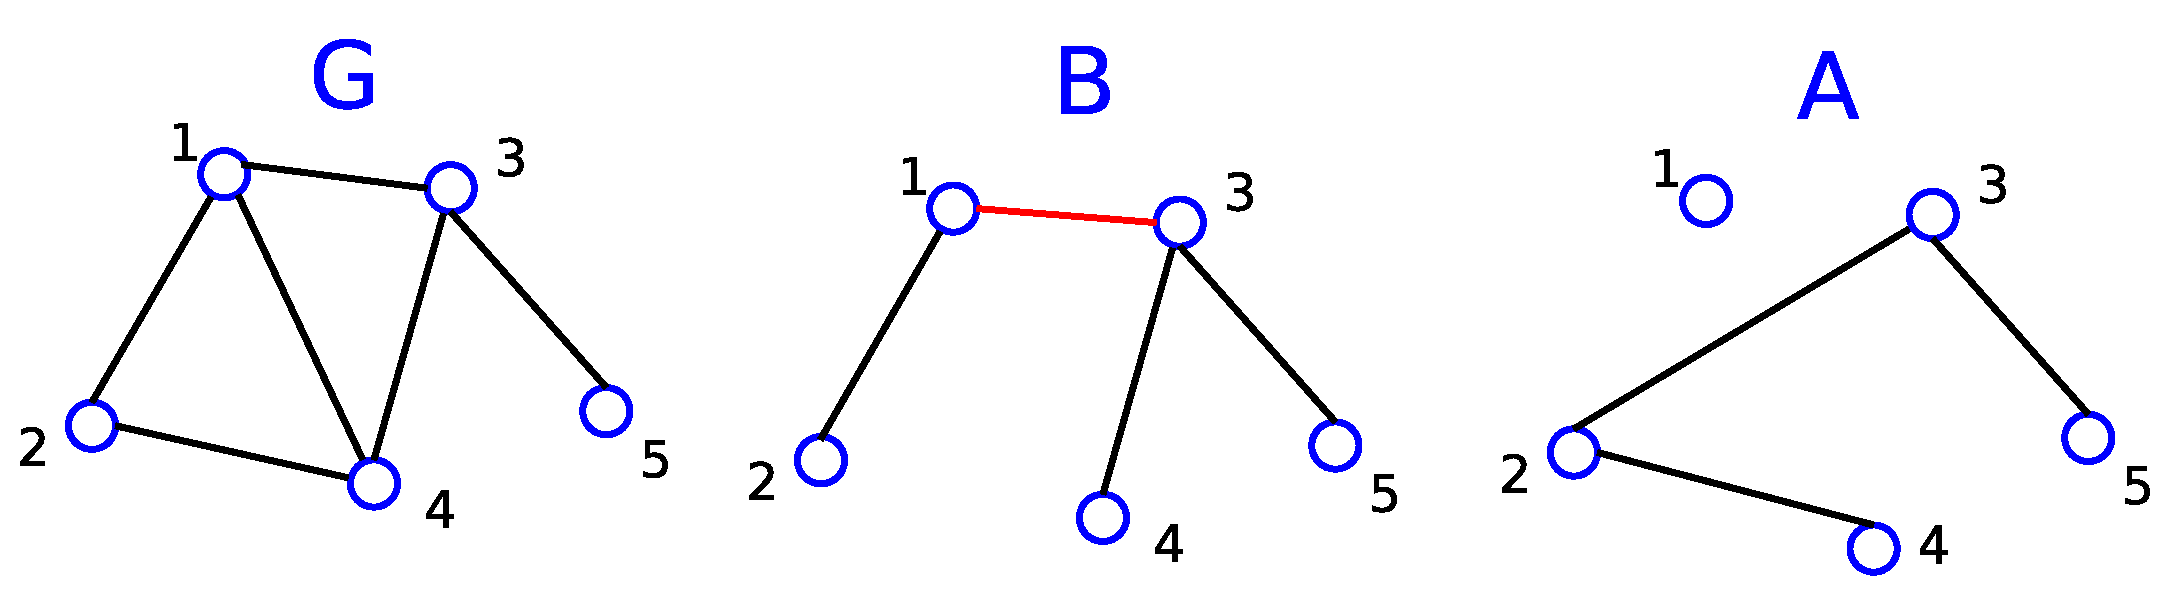
\includegraphics[width=3.3in]{L7-graphicalmatroidexample.eps}
% \end{figure}

} 

%\frame{
%\frametitle{ Why? }
%\begin{itemize}
%	\item Checking {\bf Hereditary property}: it is obvious that if a set  $B$ of edges is acyclic, any subset $A\subset B$ is also acyclic. 
%	\item Checking   {\bf Augmentation property}: 
%\end{itemize}
% \begin{figure}
% 	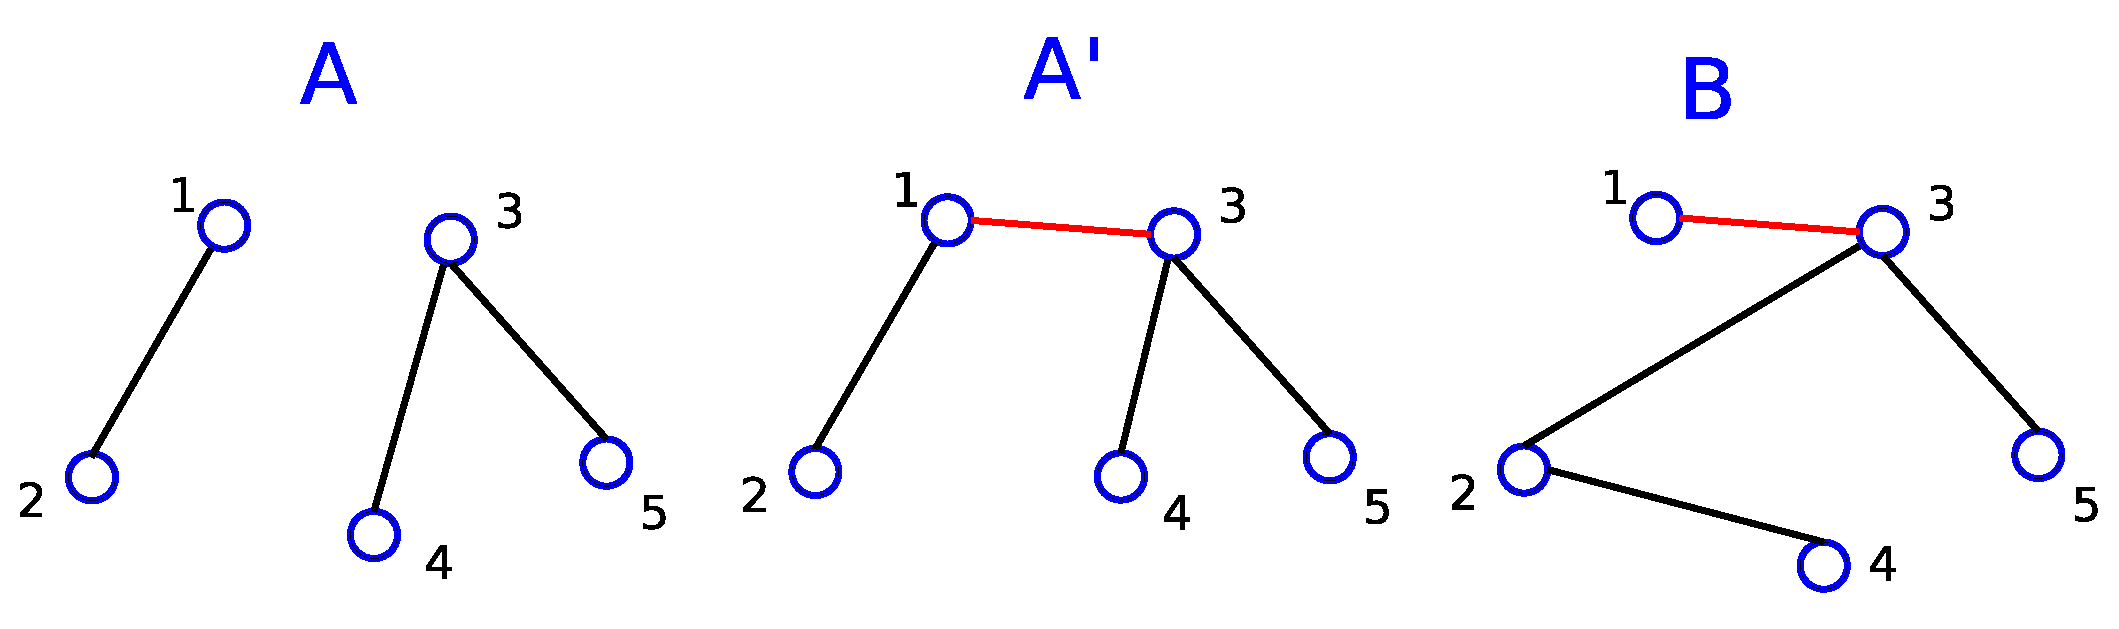
\includegraphics[width=3.3in]{L7-spanning-tree-matroid.eps}
% \end{figure}
%
%}




 \frame{
 \frametitle{Abstraction: the formal definition of matroid  }
 
 A matroid is a pair $M=(S, \mathcal{L} )$ satisfying the following conditions: 
 \begin{enumerate}
  \item $S$ is a finite nonempty set (called {\bf ground set}), and $\mathcal{L}$ is a family of {\sc independent subsets} of $S$.
  \item \textcolor{red}{\bf Hereditary property:} if $B \in \mathcal{L}$ and $A \subset B$, then $A \in \mathcal{L}$; 
  \item \textcolor{red}{\bf Augmentation property:}  if $A \in \mathcal{L}$, $B \in \mathcal{L}$, and $|A| < |B|$, then there is some element $x \in B-A$ such that $A \cup \{x\} \in \mathcal{L}$. 
 \end{enumerate}
 
 }
  
 
% \frame[allowframebreaks]{
% \frametitle{Matroid: theoretical foundation of greedy strategy}
% Note: 
% \begin{enumerate}
%  \item is useful in determining when determining whether greedy technique yields optimal solutions. 
% \item It covers many cases of practical interest. (Some exceptions: Huffman code, Interval Scheduling problems)
% \end{enumerate}
% 
% A matroid [H. Whitney, 1935] is a pair $M=(S, \mathcal{L} )$ satisfying the following conditions: 
% \begin{enumerate}
%  \item $S$ is a finite nonempty set;
%  \item Independent: $\mathcal{L}$ is a family of \textcolor{red}{independent} subsets of $S$, i.e.  if $B \in \mathcal{L}$ and $A \subset B$, then $A \in \mathcal{L}$; 
%  \item Exchange property: if $A \in \mathcal{L}$, $B \in \mathcal{L}$, and $|A| < |B|$, then there is some element $x \subset B-A$ such that $A \cup {x} \notin \mathcal{L}$. 
%  \item (Weighted): each element $x \in S$ has a strictly positive weight $w(x)$.
% \end{enumerate}
% 
% Ex. 
% \begin{figure}
% 	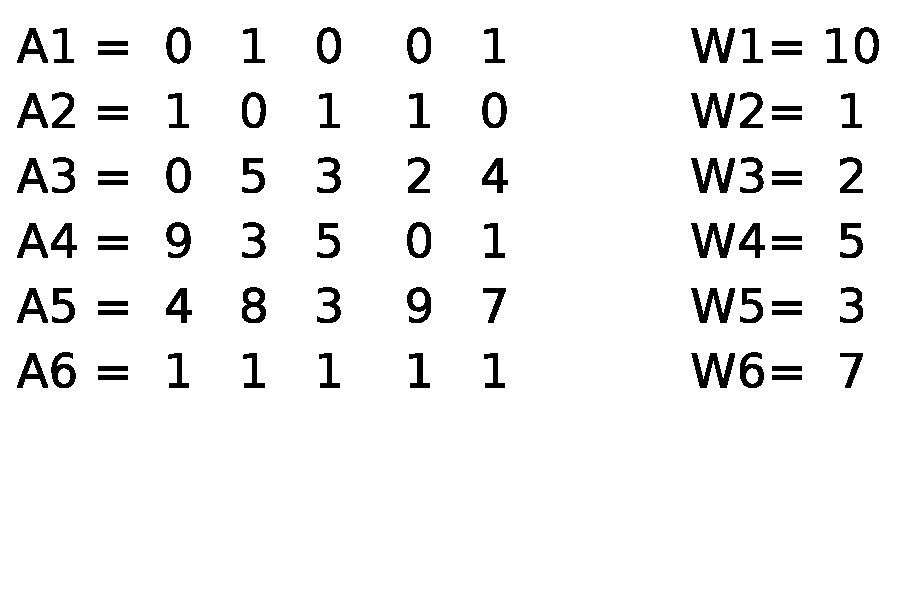
\includegraphics[width=3in]{L7-matroidexample.eps}
% \end{figure}
% }

\frame{
	\begin{block}{}
	{\sc Spanning Tree}: an application of matroid
	\end{block} 
}



\frame{
	\frametitle{ {\sc Minimum Spanning Tree} problem }
Practical problem: 
\begin{itemize}
\item In the design of electronic circuitry, it is often necessary to make the pins of several components electrically equivalent by wiring them together. 
\item To interconnect a set of $n$ pins, we can use $n-1$ wires, each connecting two pins; 
\item Among all interconnecting arrangements, the one that uses the least amount of wire is usually the most desirable. 
\end{itemize}

\begin{figure}
\begin{tikzpicture}[scale=1, auto,swap]
 
    \foreach \pos/\name in {{(0,0)/a}, {(1,1)/b}, {(1 , -1)/h}, {(2,0)/i}, {(3 ,1)/c}, {(3,-1)/g}, {(5,-1)/f},{(5,1)/d},{(6,0)/e}}
        \node[middlevertex,fill=blue!20] (\name) at \pos {$\name$};
        
    \foreach \source/\dest/\weight in {b/a/4, a/h/8, h/b/11, c/b/8, i/c/2, h/i/7, g/i/6, h/g/1, g/f/2, c/f/4, d/c/7, d/f/14, e/d/9, f/e/10 } 
            \path[undirectededge] (\source) -- node{\small $\weight$} (\dest);

    \foreach \source/\dest/\weight in {a/b/, c/i/, b/c/, c/f/, f/g/, g/h/, c/d/, d/e/  } 
            \path[selected edge] (\source) -- node{\small $\weight$} (\dest);

 
\end{tikzpicture}

\end{figure}   
} 

\frame{
	\frametitle{ {\sc Minimum Spanning Tree} problem }

Formulation: 
\begin{block}{}
{\bf Input: } A graph $G$, and each edge $e=<u, v>$ is associated with a weight $W(u, v)$;

{\bf Output: } a spanning tree with the minimum sum of weights.  Here, a spanning tree refers to a set of  $n-1$ edges  connecting all nodes. 
\end{block} 
\begin{figure}
\begin{tikzpicture}[scale=1, auto,swap]
 
    \foreach \pos/\name in {{(0,0)/a}, {(1,1)/b}, {(1 , -1)/h}, {(2,0)/i}, {(3 ,1)/c}, {(3,-1)/g}, {(5,-1)/f},{(5,1)/d},{(6,0)/e}}
        \node[middlevertex,fill=blue!20] (\name) at \pos {$\name$};
        
    \foreach \source/\dest/\weight in {b/a/4, a/h/8, h/b/11, c/b/8, i/c/2, h/i/7, g/i/6, h/g/1, g/f/2, c/f/4, d/c/7, d/f/14, e/d/9, f/e/10 } 
            \path[undirectededge] (\source) -- node{\small $\weight$} (\dest);

    \foreach \source/\dest/\weight in {a/b/, c/i/, b/c/, c/f/, f/g/, g/h/, c/d/, d/e/  } 
            \path[selected edge] (\source) -- node{\small $\weight$} (\dest);

 
\end{tikzpicture}

\end{figure}   


}


\frame{
	\frametitle{  {\sc Independent Vector Set} versus {\sc Acyclic Forest} } 
	
	 \begin{figure}
 	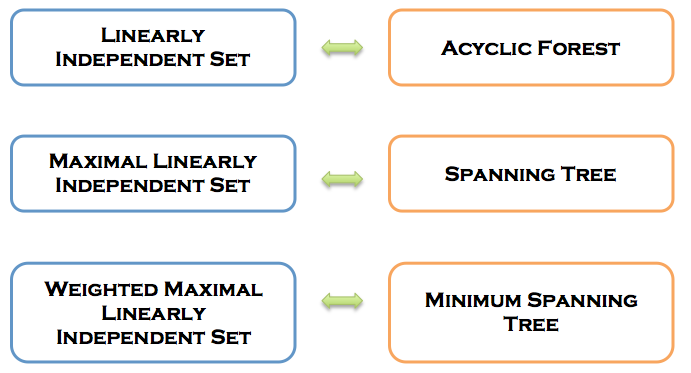
\includegraphics[width=4in]{L7-independentsetforest.png}
 \end{figure}
}


\frame{
	\frametitle{ {\sc Generic Spanning Tree} algorithm } 

\begin{itemize}
\item Objective: to find a spanning tree for graph $G$; 
\item Basic idea: analogue to {\sc Maximal Linearly Independent Set} calculation; 
\end{itemize}


{\sc GenericSpanningTree}$( G )$
\begin{algorithmic}[1]
\STATE{ $F=\{ \};$ }
\WHILE{ $F$ does not form a spanning tree } 
\STATE{ find an edge $(u, v)$ that is \textcolor{red}{\bf safe} for $F$; }
\STATE{ $F = F\cup\{ (u, v) \}$; }
\ENDWHILE
\end{algorithmic}
	
	Here $F$ denotes an {\sc acyclic forest}, and  $F$ is still {\sc acyclic} if added by a \textcolor{red}{\bf safe} edge. 
}

\frame{
	\frametitle{ Examples of safe edge and unsafe edge}
\begin{figure}
\begin{tikzpicture}[scale=1, auto,swap]
 
    \foreach \pos/\name in {{(0,0)/a}, {(1,1)/b}, {(1 , -1)/h}, {(2,0)/i}, {(3 ,1)/c}, {(3,-1)/g}, {(5,-1)/f},{(5,1)/d},{(6,0)/e}}
        \node[middlevertex,fill=blue!20] (\name) at \pos {$\name$};
        
    \foreach \source/\dest/\weight in {b/a/4, a/h/8, h/b/11, c/b/8, i/c/2, h/i/7, g/i/6, h/g/1, g/f/2, c/f/4, d/c/7, d/f/14, e/d/9, f/e/10 } 
            \path[undirectededge] (\source) -- node{\small $\weight$} (\dest);

    \foreach \source/\dest/\weight in {a/b/, c/i/, c/f/,  f/g/  } 
            \path[selected edge] (\source) -- node{\small $\weight$} (\dest);

    \foreach \source/\dest/\weight in {c/d/ } 
            \path[undirectededge, blue, ultra thick] (\source) -- node{\small $\weight$} (\dest);

\end{tikzpicture} 
\caption{Safe edge} 
\end{figure}   

\begin{figure}
\begin{tikzpicture}[scale=1, auto,swap]
 
    \foreach \pos/\name in {{(0,0)/a}, {(1,1)/b}, {(1 , -1)/h}, {(2,0)/i}, {(3 ,1)/c}, {(3,-1)/g}, {(5,-1)/f},{(5,1)/d},{(6,0)/e}}
        \node[middlevertex,fill=blue!20] (\name) at \pos {$\name$};
        
    \foreach \source/\dest/\weight in {b/a/4, a/h/8, h/b/11, c/b/8, i/c/2, h/i/7, g/i/6, h/g/1, g/f/2, c/f/4, d/c/7, d/f/14, e/d/9, f/e/10 } 
            \path[undirectededge] (\source) -- node{\small $\weight$} (\dest);

    \foreach \source/\dest/\weight in {a/b/, c/i/, c/f/, f/g/ } 
            \path[selected edge] (\source) -- node{\small $\weight$} (\dest);

    \foreach \source/\dest/\weight in {g/i/ } 
            \path[undirectededge, blue, ultra thick] (\source) -- node{\small $\weight$} (\dest);

\end{tikzpicture}
\caption{Unsafe edge}  
\end{figure}   
}



\frame{
	\begin{block}{}
	{\sc Minimum Spanning Tree} algorithms
	\end{block}
}







\frame{
\frametitle{ Kruskal's algorithm [1956]  }

\begin{itemize}
\item Basic idea:  during the execution, $F$ is always an \textcolor{red}{\bf acyclic forest}, and the \textcolor{red}{\bf safe edge} added to $F$ is always a least-weight edge connecting two distinct components. 
\end{itemize}
\begin{figure}
     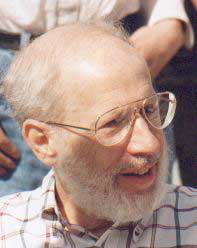
\includegraphics[width=1.5in]{Kruskal.png}
 \caption{ Joseph Kruskal} 
\end{figure}
} 

%
%
%
%\item 
%For graph $G$, we first construct its {\sc graphic matroid} $M_{G}=( S_G, {L} _G)$ as follows: 
%\begin{enumerate}
% \item {\sc Ground set: }  $S_G = E$, the set of edges; 
% \item {\sc Independent subsets:}  $A \in \mathcal{L}_G$ iff $A$ is acyclic. (Intuition: $A$ forms a forest, i.e.  a set of trees.)
% \item Weight: $w(e) = W_{max} - C(e)$, where $W_{max}$ is a large number to guarantee $w(e) > 0 $; 
%\end{enumerate}
%
%\item  
%Since $M_{G}$ is a matroid, the general {\sc Matroid\_Greedy} algorithm also applies: Kruskal's algorithm.
%\end{itemize}
%}

\frame{
\frametitle{ Kruskal's algorithm   [1956]}

{\sc MST-Kruskal}$( G, W )$
\begin{algorithmic}[1]
\STATE{ $F = \{ \}; $} 
\FORALL{ vertex $v \in V$ } 
\STATE{ {\sc MakeSet}$( v )$; }
\ENDFOR
\STATE\textcolor{red}{ sort the edges of $E$ into nondecreasing order by weight $W$; }
\FOR{ each edge $(u, v) \in E$ in the order } 
\IF { {\sc FindSet}$( u )$ $\neq$ {\sc FindSet}$( v )$ } 
\STATE $F = F \cup \{ ( u , v ) \};$ 
\STATE{{\sc Union} $( u, v )$; } 
\ENDIF
\ENDFOR
\end{algorithmic}

Here,  {\sc Union-Find} structure is used to detect whether a set of edges form a cycle. 

(See extra slides for {\sc Union-Find} data structure, and a demo of Kruskal algorithm)
} 

\frame{
\frametitle{ Time complexity }

\begin{itemize} 
 \item Running time: 
	\begin{enumerate}
	 \item Sorting: $O(m \log m)$
	 \item Initializing: $n$ {\sc MakeSet} operations;  
	 \item Detecting cycle: $2m$ {\sc FindSet} operations; 
	 \item Adding edge: $n-1$ {\sc Union} operations. 
		\end{enumerate}
\end{itemize}

\begin{itemize} 
\item 
Thus, the total time is $O( (m+n) \alpha(n) )$, where $\alpha(n)$ is a very slowly growing function. 
\item Since $\alpha(n) = O(\lg n )$, the total running time is $O( m \lg n )$. 
\end{itemize} 
}

\frame{
	\begin{block}{}
	 Prim's algorithm
	\end{block}
}

\frame{
	\frametitle{ Prim's algorithm  [1957]} 
	\begin{itemize}
	\item Basic idea: the final minimum spanning tree is grown step by step. At each step, the least-weight edge connect the sub-tree to a node not in the tree is chosen. 	
	\item Note: 
		One advantage of Prim's algorithm is that no special check to make sure that a cycle is not formed is required.
	\end{itemize}
	
	\begin{figure}
     \includegraphics[width=1.3in]{Prim.png}
 \caption{ Robert C. Prim} 
\end{figure}
} 

\frame{
	\frametitle{Greedy selection property} 
\begin{Theorem}{[Greedy selection property]}
Suppose $T$ is a sub-tree of the final minimum spanning tree, and $e=(u,v)$ is the least-weight edge connect one node in $T$ and another node not in $T$. Then $e$ is in  the final minimum spanning tree. 
 \end{Theorem}
 
 \begin{figure}
\begin{tikzpicture}[scale=1, auto,swap]
 
   \node[red, ultra thick] at (3, 1.5) {$root$};
    \foreach \pos/\name in {{(0,0)/a}, {(1,1)/b}, {(1 , -1)/h}, {(3,-1)/g}, {(5,1)/d},{(6,0)/e}}
        \node[middlevertex,fill=blue!20] (\name) at \pos {$\name$};
  
      \foreach \pos/\name in {{(2,0)/i}, {(3 ,1)/c}, {(5,-1)/f}}
        \node[middlevertex,fill=yellow] (\name) at \pos {$\name$};
        
              
    \foreach \source/\dest/\weight in {b/a/4, a/h/8, h/b/11,  i/c/2,   h/g/1, g/f/2, c/f/4,   e/d/9 } 
            \path[undirectededge] (\source) -- node{\small $\weight$} (\dest);

    \foreach \source/\dest/\weight in {c/i/,  c/f/ } 
            \path[selected edge, fill=yellow] (\source) -- node{\small $\weight$} (\dest);
            
      \foreach \source/\dest/\weight in {c/b/8,  d/c/7, h/i/7, g/i/6, d/f/14, f/e/10 } 
            \path[undirectededge, dashed, blue] (\source) -- node{\small $\weight$} (\dest);
                      
    \foreach \source/\dest/\weight in {g/f/ } 
            \path[undirectededge, blue, ultra thick] (\source) -- node{\small $\weight$} (\dest);

 
 
\end{tikzpicture}
\end{figure} 

}

\frame{
	\frametitle{ {\sc Prim} algorithm for {\sc Minimum Spanning Tree} [1957] }
{\sc MST-Prim}$( G, W, root )$
\begin{small}
\begin{algorithmic}[1]
\FORALL{ node $v \in V$ and $v \neq root$ } 
\STATE{ $key[v] = \infty;$}
\STATE{ $\Pi[v] = $ {\sc Null};  //$\Pi(v)$ denotes the predecessor node of $v$ }
\STATE{ $PQ.${\sc Insert}$( v )$;  \textcolor{red}{// n times} }
\ENDFOR
\STATE{ $key[ root ] = 0;$ }
\STATE{ $PQ.${\sc Insert}$( root )$;}
\WHILE{ $PQ \neq $ {\sc Null} }
\STATE{  $u = PQ.${\sc ExtractMin}$()$; \textcolor{red}{// n times} } 
\FORALL{ $v$ adjacent with $u$ } 
\IF { $W(u, v) < key(v)$} 
\STATE $\Pi( v ) = u $; 
\STATE $PQ.${\sc DecreaseKey}$(  W(u, v) )$; \textcolor{red}{// m times}
\ENDIF
\ENDFOR
\ENDWHILE
\end{algorithmic}
Here, $PQ$ denotes a min-priority queue. The chain of predecessor nodes originating from $v$ runs backwards along a shortest path from $s$ to $v$.  

(See a demo)
\end{small}
}

\frame{
	\frametitle{ Time complexity of {\sc Prim} algorithm} 

  \begin{table}
  \begin{tabular}{crrrr}
  \hline  \hline
  Operation & Linked  & Binary  & Binomial  & Fibonacci  \\
            &  list &  heap &  heap & heap \\
  \hline
  {\sc MakeHeap} & $ 1 $ &  $1$  & $ 1 $ & $1$  \\ 
  {\sc Insert} & $ 1 $ &  $\log n$  & $ \log n $ & $1$  \\ 
   {\sc ExtractMin} & $ n $ &  $\log n$  & $ \log n  $ & $ \log n $  \\ 
  {\sc DecreaseKey} & $ 1 $ &  $\log n$  & $ \log n $ & $1$  \\ 
  {\sc Delete} & $ n $ &  $\log n$  & $ \log n $ & $\log n$  \\ 
  {\sc Union} & $ 1 $ &  $ n $  & $ \log n $ & $1$  \\ 
   {\sc FindMin} & $ n $ &  $1$  & $ \log n $ & $1$  \\ 
  \hline 
  {\sc Prim} & $ O(n^2) $ &  $ O(m \log n) $  & $ O( m \log n ) $ & $ O( m + n \log n) $  \\ 
  \hline \hline 
  \end{tabular} 
  \end{table}
{\sc Prim} algorithm: $n$ {\sc Insert}, $n$ {\sc ExtractMin}, and $m$ {\sc DecreaseKey}. 
}





\frame{ 
\frametitle{ Applications of Matroid } 
Note: 
 \begin{enumerate}
  \item Matroid is useful when determining whether greedy technique yields optimal solutions. 
 \item It covers many cases of practical interests (Some exceptions: Huffman code, Interval Scheduling problems).
 \end{enumerate}
} 



\frame{
\begin{block}{}
{\sc Huffman Code} 
\end{block}
}


\frame{
\frametitle{Compressing files }

\begin{itemize} 
\item 
Practical problem: how to compact a file when you have the knowledge of frequency of letters? 
\item 
Example: 
\begin{footnotesize}
\begin{table}{
\begin{tabular}{lllllllll} 
\hline
SYMBOL & \texttt{A} & \texttt{B} & \texttt{C} & \texttt{D} & \texttt{E}  &\\
Frequency & 24 & 12 & 10 & 8 & 8 & \\ 
Fixed Length Code & \texttt{000} & \texttt{001} &\texttt{010} &\texttt{011} &\texttt{100} & $E(L)=186$ \\
Variable Length Code & \texttt{00} & \texttt{01} &\texttt{10} &\texttt{110} &\texttt{111}& $E(L)=140$ \\
\hline
\end{tabular} } {} 
\end{table} 
\end{footnotesize}
\end{itemize} 
}

\frame{
\frametitle{ Formulation }

\begin{block}{}
 {\bf INPUT: } \\a set of symbols $S=\{s_1, s_2, ..., s_n\}$ with its appearance frequency $P=\{p_1, p_2, ..., p_n\}$; \\ 
 {\bf OUTPUT: } \\assign each symbol with a binary code $C_i$ to minimize the length expectation $\sum_i p_i | C_i |$.  
\end{block}
} 


\frame[allowframebreaks]{
\frametitle{Requirement: prefix code}

\begin{itemize}
 \item 
 To avoid the potential ambiguity in decoding, we require the coding to be {\bf prefix code}. 
 \begin{definition}[Prefix coding] 
A prefix coding for a symbol set $S$ is a coding such that for any symbols $x, y \in S$,  the code $C(x)$ is not prefix of the code $C(y)$. 
\end{definition}
\item
Intuition: A prefix code can be represented as a binary tree, where a leaf represents a symbol, and the path to a leaf represents the code. 
\item
Our objective: to design an optimal tree $T$ to minimize expected length $E(T)$ (the size of the compressed file). 
\end{itemize}

\begin{figure}
	\includegraphics[width=3.95in]{L7-prefixcode.eps}
\end{figure}
}

%\frame{ 
%\frametitle{ We need a complete tree!}
%\begin{figure} 
% \includegraphics[width=4in]{binarytree.eps}
%\end{figure}
%} 

\frame{
\frametitle{ Full binary tree}
\begin{Theorem}{}
 An optimal binary tree should be a full tree. 
\end{Theorem}
\begin{Proof}
\begin{itemize}
 \item 
 Suppose $T$ is an optimal tree but is not full; \\
\item There is a node $u$ with only one child $v$; \\
\item Construct a new tree $T'$, where $u$ is replaced with $v$; 
\item $E(T') \leq E(T)$ since any child of $v$ has a shorter code. 
\end{itemize}
\end{Proof}

\begin{figure}
	\includegraphics[width=2.2in]{L7-prefixcodefulltree.eps}
\end{figure}
}

\frame{
	\begin{block}{}
Top-down manner: a false start
	\end{block} 
} 

\frame{
\frametitle{ Shannon-Fano coding  [1949] }
Top-down method : 
\begin{algorithmic}[1]
\STATE Sorting $S$ in the decreasing order of frequency. 
\STATE Splitting $S$ into two sets $S_1$ and $S_2$ with almost equal frequencies. 
\STATE Recursively building trees for $S_1$ and $S_2$. 
\end{algorithmic}

\begin{figure}
 \begin{minipage}{0.40\textwidth}
     \includegraphics[width=0.8\textwidth]{Shannon.jpg}
 \end{minipage}
 \begin{minipage}{0.40\textwidth}
     \includegraphics[width=1.0\textwidth]{Fano.jpg}
 \end{minipage}
 \caption{ Claude Shannon and Robert Fano} 
\end{figure}
}

\frame{
\frametitle{ An example: Step 1}

\begin{figure}
     \includegraphics[width=2.7in]{L7-ShannonFano-all.png}
\end{figure}
\begin{figure}
     \includegraphics[width=2in]{L7-ShannonFano-step1.png}
\end{figure}
}

\frame{
\frametitle{ An example: Step 2}

\begin{figure}
     \includegraphics[width=2.7in]{L7-ShannonFano-all.png}
\end{figure}
\begin{figure}
     \includegraphics[width=2.3in]{L7-ShannonFano-step2.png}
\end{figure}
}


\frame{
\frametitle{ An example: Step 3}

\begin{figure}
     \includegraphics[width=2.7in]{L7-ShannonFano-all.png}
\end{figure}
\begin{figure}
     \includegraphics[width=2.8in]{L7-ShannonFano-step3.png}
\end{figure}
}

\frame{
	\begin{block}{}
Bottom-up manner
	\end{block} 
} 

\frame{
\frametitle{ Huffman code: bottom-up manner [1952] }

Bottom-up method: 
\begin{algorithmic}[1]
\REPEAT
\STATE Merging the two lowest-frequency letters $y$ and $z$ into a new meta-letter $yz$,
\STATE  Setting $P_{yz} = P_y + P_z $.  
\UNTIL{only one label is left} 
\end{algorithmic}
\begin{figure}
     \includegraphics[width=1.3in]{Huffman.png}
\end{figure}

} 

\frame{
\frametitle{ Huffman code: bottom-up manner [1952] }

Key Observations: 
\begin{enumerate}
 \item In an optimal tree, $depth(u) \geq depth(v)$ iff $P_u \leq P_v$. (Exchange argument)
 \item There is an optimal tree, where the lowest-frequency letters $Y$ and $Z$ are siblings. 
  (Why?) \begin{itemize}
              \item Consider a deepest node $v$.
              \item $v$'s parent, denoted as $u$, should has another child, say $w$. 
              \item $w$ should also be a deepest node. 
              \item $v$ and $w$ have the lowest frequency. 
  	     \end{itemize}
\end{enumerate}
}

\frame{
\frametitle{ Huffman code algorithm 1952}
{\sc Huffman}$( S, P )$
\begin{algorithmic}[1]
\IF { $| S | == 2 $}
\RETURN a tree with a root and two leaves; 
\ENDIF
\STATE Extract the two lowest-frequency letters $Y$ and $Z$ from $S$;
\STATE Set $P_{YZ}=P_Y+P_Z$;
\STATE $S=S-\{Y,Z\}\cup \{YZ\}$;
\STATE $T'=${\sc Huffman}$(S, P)$;
\STATE $T=$ add two children $Y$ and $Z$ to node $YZ$ in $T'$;
\RETURN $T$;
\end{algorithmic}
}


\frame{
\frametitle{Example}
\begin{figure}
	\includegraphics[width=2.5in]{L7-Huffmantree.png}
\end{figure}
\begin{figure}
	\includegraphics[width=2.5in]{L7-Huffmantreecode.png}
\end{figure}
}

\frame{
\frametitle{Shannon-Fano vs. Huffman}

\begin{figure}
 \begin{minipage}{0.45\textwidth}
     \includegraphics[width=1.0\textwidth]{L7-ShannonFano-step3.png}
 \end{minipage}
 \begin{minipage}{0.42\textwidth}
     \includegraphics[width=1.0\textwidth]{L7-Huffmantree.png}
 \end{minipage}
\end{figure}
\begin{figure}
	\includegraphics[width=2.5in]{L7-ShannonFanoHuffman.png}
\end{figure}
}




\frame{
\frametitle{ Huffman algorithm:  correctness }

\begin{lemma}
 $E(T') = E(T) - P_{YZ}$
\end{lemma}
\begin{footnotesize}  
\begin{Proof}
\begin{eqnarray}
 E(T) &=& \sum_{x \in S } P_x  D( x, T) \nonumber\\ 
&=& P_Y D( Y, T) + P_Z D( Z, T) +  \sum_{x \neq Y, x\neq Z} P_x D( x, T) \nonumber\\
&=& P_Y ( 1 + D( YZ, T') ) + P_Z ( 1 + D( YZ, T') ) +  \sum_{x \neq Y, x\neq Z} P_x D( x, T) \nonumber\\  
&=& P_{YZ} + P_Y D( YZ, T') + P_Z  D( YZ, T') +  \sum_{x \neq Y, x\neq Z} P_x D( x, T') \nonumber\\
&=& P_{YZ} + E(T') \nonumber
\end{eqnarray}
\end{Proof}
Note: $D(x, T)$ denotes the depth of leaf $x$ in tree $T$. 
\end{footnotesize} 
}

\frame{
\frametitle{ Huffman algorithm:  correctness  cont'd}


\begin{Theorem}
Huffman algorithm output an optimal code. 
\end{Theorem}
\begin{Proof} (Induction)
\begin{itemize}
 \item 
Suppose there is another tree $t$ with smaller expected length; \\
\item 
In the tree $t$, let's merge the lowest frequency letters $Y$ and $Z$ into a meta-letter $YZ$; converting $t$ into a new tree $t'$ with of size $n-1$;  \\
\item 
$t'$ is better than $T'$. Contradiction. 
\end{itemize}
\end{Proof}

}



\frame{
\frametitle{ Analysis }

Time complexity: 
\begin{itemize}
 \item 
$T(n) = T(n-1) + O(n) = O(n^2)$.
\item 
$T(n) = T(n-1) + O(\log n ) = O(n \log n)$ if use priority queue. 
\end{itemize}

Note: Huffman code is a bit different example of greedy technique---the problem is shrinked at each step; in addition, the problem is changed a little (the frequency of a new meta letter is the sum frequency of its members).
} 

\frame{
\frametitle{ Application  }
 \begin{itemize} 
 \item In practical operation Shannon-Fano coding is not of larger importance. This is especially caused by the lower code efficiency in comparison to Huffman coding. 
 \item 
Huffman codes are part of several data formats as ZIP, GZIP and JPEG. Normally the coding is preceded by procedures adapted to the particular contents. For example the wide-spread DEFLATE algorithm as used in GZIP or ZIP previously processes the dictionary based LZ77 compression.
 \end{itemize} 
 See http://www.binaryessence.com/dct/en000003.htm for details. 
} 



\end{document}
